%                                                                 aa.dem
% AA vers. 9.1, LaTeX class for Astronomy & Astrophysics
% demonstration file
%                                                       (c) EDP Sciences
%-----------------------------------------------------------------------
%
%\documentclass[referee]{aa} % for a referee version
%\documentclass[onecolumn]{aa} % for a paper on 1 column  
%\documentclass[longauth]{aa} % for the long lists of affiliations 
%\documentclass[letter]{aa} % for the letters 
%\documentclass[bibyear]{aa} % if the references are not structured 
%                              according to the author-year natbib style

%===========% DATE RENDU : 23 Novembre 2023 %===========mj

%
\documentclass{aa}  
%%%%%%%%%%%%%%%%%%%%%%%%%%%%%%%%%%%%%%%%
\usepackage{graphicx} % Required for inserting images
\usepackage[french]{babel}
\usepackage[T1]{fontenc}
\selectlanguage{french}
\usepackage[utf8]{inputenc}
\usepackage{amsmath}
\usepackage{amsfonts,amsthm, amssymb}
\usepackage{esvect}
\usepackage{array}
%\usepackage[top=2cm,bottom=2cm,left=2cm,right=2cm]{geometry}
\graphicspath{./images/}
\usepackage{hyperref}

%%%%%%%%%%%%%%%%%%%%%%%%%%%%%%%%%%%%%%%%
%\usepackage[options]{hyperref}
% To add links in your PDF file, use the package "hyperref"
% with options according to your LaTeX or PDFLaTeX drivers.
%
\begin{document} 


   \title{Déterminer la masse de Jupiter grâce à la troisième loi de Kepler}

   \author{Justin Peret\inst{1} et
          Antonin Pelletier\inst{2}
          }

   \institute{L3 Magistère de Physique, Université Paris-Cité, France\\
              \email{justin.peret@etu.u-paris.fr}
         \and
             L3 Magistère de Physique, Université Paris-Cité, France\\
             \email{antonin.pelletier@etu.u-paris.fr}
             }

   \date{Date de dépôt: Mercredi 20 Décembre 2023}

% \abstract{}{}{}{}{} 
% 5 {} token are mandatory
 
  \abstract
  % context heading (optional)
  % {} leave it empty if necessary  
   { Après une démonstration mathématique des trois lois de Kepler, nous cherchons à montrer par de multiples séries d'observations que la loi des périodes - troisième loi - est valable dans le cadre de Jupiter et de ses satellites galiléens. Nous utilisons ensuite nos observations afin de donner une approximation de la masse de Jupiter, ce en utilisant l'expression de la troisième Loi de Kepler et la constante k obtenue expérimentalement.} 
  % aims heading (mandatory)
  % {}
  % methods heading (mandatory)
  % {}
  % results heading (mandatory)
  % {}
  % conclusions heading (optional), leave it empty if necessary 
  % {}

   \keywords{ Kepler, Jupiter, Loi, Satellites, Orbite, Ellipse
               }

   \maketitle
%
%-------------------------------------------------------------------

\section{Introduction}
%\begin{flushleft}
    L'étude des astres visibles dans notre ciel nocturne est historiquement la raison d'être de l'astronomie, qui leur a accordé une place centrale durant des centaines d'années. Kepler, qui s'est intéressé aux "astres errants", a établi sur la base des travaux de \emph{Tycho Brahe} \textbf{[1]} trois lois qui portent désormais son nom. Ces lois stipulent que les planètes du système solaire décrivent une trajectoire elliptique dont le Soleil est un foyer, qu’en des temps égaux elles balaient des aires égales et enfin que leur période de révolution est proportionnelle à leur demi-grand axe avec un coefficient de proportionnalité identique pour toutes les planètes. \\
    Les trois lois de Kepler ont originellement été énoncées pour le Soleil mais sont communément admises comme valables et utilisées - à juste titre - pour n'importe quel astre du système solaire.\\
    On se propose ici de démontrer expérimentalement la troisième loi de Kepler en utilisant Jupiter et les quatre satellites galiléens Io, Europe, Callisto et Ganymède. Nous considérerons la période de révolution de chacun des ces satellites comme connue \textbf{[2]}.\\
    
    À partir de la troisième loi de Kepler et en négligeant la masse des satellites galiléens devant celle de Jupiter (le rapport de $10^5$ kg entre les deux justifie cette approximation), on pourra également obtenir une approximation de la masse de Jupiter.
    
    
%\end{flushleft}

%--------------------------------------------------------------------
\section{Modélisation \& Théorie}

%\subsection{Positionnement du problème}
% Phénomènes et Explications


\subsection{Lois de Kepler}
% Enoncés des lois ( et provenance ?)
Ces lois sont essentielles afin d'appréhender le comportement des planètes .En effet, elles posent les bases de leur comportement et nouent ou dénouent des liens entre différents phénomènes et caractéristiques des astres telles que leur trajectoire, leur masse etc... Ces lois sont au nombre de trois. On introduit pour plus de clarté dans les lois quantitatives les notations suivantes: \break

\begin{itemize}
    \item $m_S$ la masse du Soleil \\
    \item $m_P$ la masse de la planète P orbitant autour du Soleil \\
    \item $\vv{SP}$ le vecteur position de la planète par rapport au Soleil. \\ 
    \item $r$ la norme du vecteur $\vv{SL}$ \\
    \item $\theta$ l'angle du vecteur $\vv{SL}$ par rapport à l'axe $\left(Sx\right)$ orienté dans le sens positif.\\
    \item $G$ la constante de gravitation universelle. \\
    \item $p$ le paramètre de l'ellipse tel que $\left[p\right] = 1 $ \\
    \item $e$ l'excentricité de l'ellipse tel que $\left[e\right] = 1 $ \\
    \item $\vv{v}$ la vitesse de la planète P par rapport au Soleil, de norme $v = \| \vv{v} \|$ \\
    \item $\vv{\sigma}_S$ le moment cinétique de $P$ autour du point fixe $S$ \\
    \item $a$ le demi-grand axe de l'ellipse \\
    \item $b$ le demi-petit axe de l'ellipse  \\
    \item $C$ la constante des aires \\
\end{itemize}

\begin{center}
    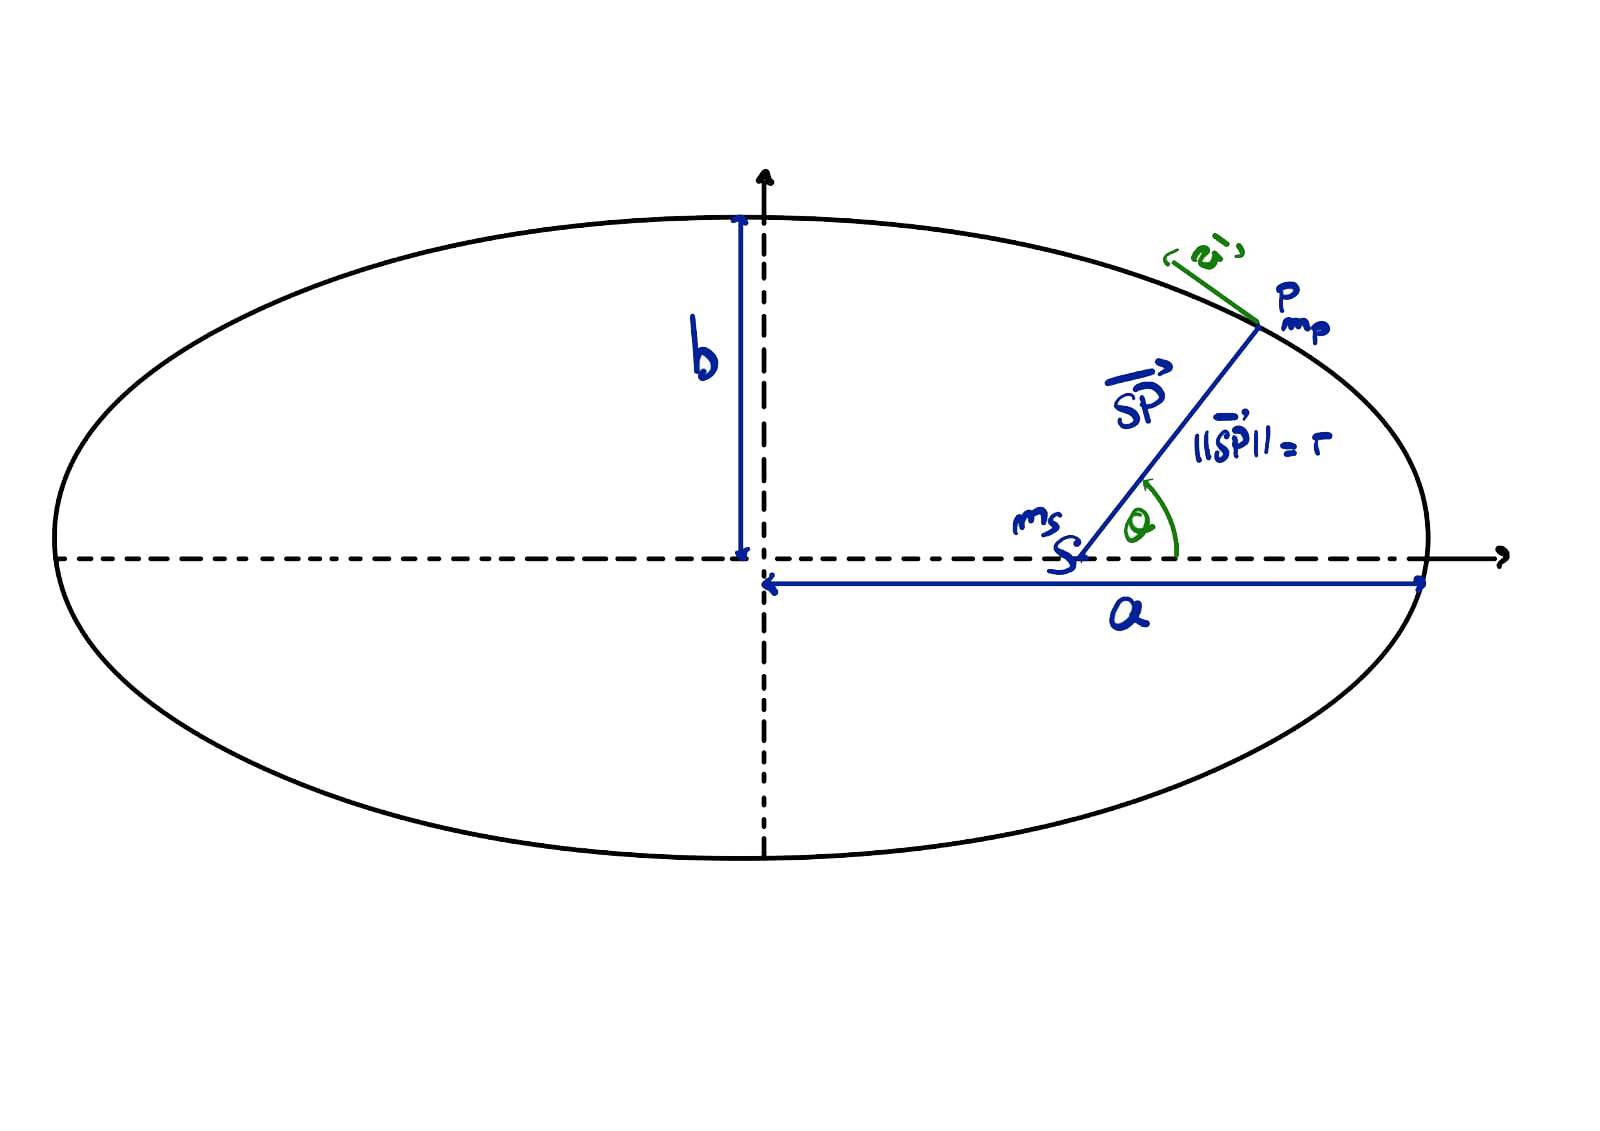
\includegraphics[scale = 0.17]{images/schema ellipse intro notions png.png} \\
    \emph{\textbf{Figure 0.} Schema représentatif de l'orbite d'une planète autour du Soleil et les notations associées}
\end{center}


\begin{flushleft}
\textit{\textbf{Première Loi de Kepler : Des Orbites}} \\    
\end{flushleft}
La première loi énonce que la trajectoire décrite par les planètes du système solaire est elliptique. \\
Comme la seule force s'appliquant sur les planètes est l'attraction gravitationnelle du Soleil sur les planètes et que celle-ci est conservative, son énergie mécanique est conservée. Ainsi après un calcul sur celle-ci (cf. annexe), on obtient un rayon $r$ qui varie en fonction de $\theta$ : $r(\theta)$ exprimé par: \\

\begin{equation}
    r(\theta) = \frac{p}{1 + ecos(\theta)}
\end{equation}

Qui décrit bien une ellipse pour $0 < e < 1$ et un cercle pour $e=0$ et où $p = \frac{b}{a}$. \\

On obtient également une expression de la constante des aires C: 

\begin{equation}
    C^{2} = Gm_Sp 
\end{equation}


\begin{flushleft}
\textit{\textbf{Deuxième Loi de Kepler: Des Aires}} \\    
\end{flushleft}

La seconde loi de Kepler livre qu'en des durées égales, les aires balayées par le vecteur position d'une planète autour du Soleil sont les mêmes. Cela implique alors que la vitesse de la planète n'est pas la même sur l'entièreté de son orbite. Par exemple elle sera plus élevée au périhélie qu'a l'aphélie. Plus généralement la vitesse est inversement proportionnelle à l'altitude $r$: $v \propto \frac{1}{r}$

\begin{center}
    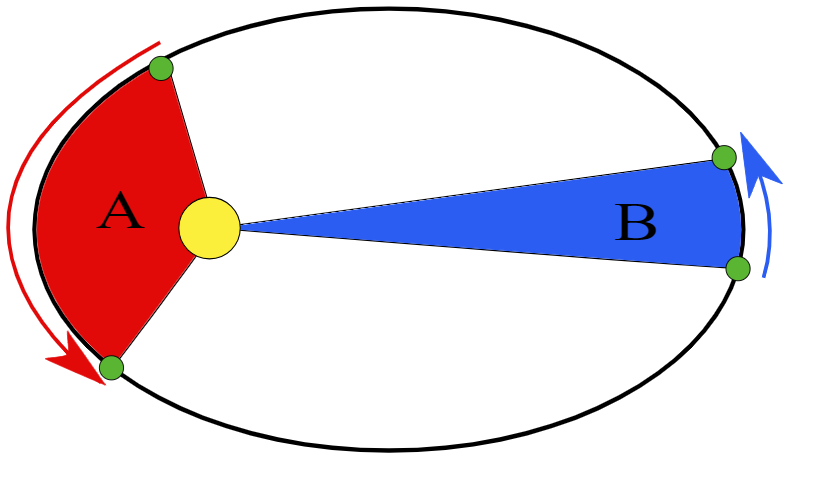
\includegraphics[scale = 0.4]{images/loi des aires.png} \\
    \emph{\textbf{Figure 1.} Illustration de la loi des aires \textbf{[3]}}
\end{center}

On la démontre en calculant le moment cinétique $\vv{\sigma}_S$ et en le reliant à l'aire. On obtient alors la constante des aires (cf. annexe): 
\begin{equation}
    A_t = \frac{C}{2}t 
\end{equation}

Où $C^2 = r^2\frac{d\theta}{dt}$ et ainsi l'aire balayée lors d'un temps t ne dépend que de C qui est constante.

\begin{flushleft}
\textit{\textbf{Troisième Loi de Kepler: Des Périodes}} \\    
\end{flushleft}

La troisième loi livre que le rapport du demi-grand axe élevé au carré et de la période de rotation de la planète élevée au cube est une constante. On la démontre en utilisant les deux premières lois sur une période de rotation T et une expression alternative de $C$ en fonction de $G$, $m_S$ et $p$ via la première loi pour finalement obtenir (cf.annexe) :

\begin{equation}
    \frac{T^2}{a^3} = \frac{4 \pi ^2}{Gm_S} = k
\end{equation}

Cette loi relève la présence d'une certaine harmonie dans le système solaire étant donné que ce rapport est une constante \emph{k} ne dépendant que de la masse du système central ( et non de celle de l'astre en orbite ) et de la constante de gravitation universelle mais est surtout commune à tout astre orbitant autour du Soleil.

\subsubsection{Résultats Théoriques Attendus}

On calculera dans cette partie les résultats théoriques attendus, c'est-à-dire la valeur de $\frac{T^2}{a^3}$ et la masse de Jupiter $m_J$. \\

On prend arbitrairement la période et le demi-grand axe de l'ellipse associée à Europe:\\

\item - $a_{europe} = 671 000$ km \\
\item - $T_{europe} = 85$ h \\

On obtient alors: 
\begin{equation}
    \frac{T_{europe}^2}{a_{europe}^3} = 3.12\times10^{-16} \quad s^2m^{-3}
\end{equation}

Ce qui livre directement la masse de Jupiter:

\begin{equation}
    m_J = \frac{4\pi^2a^3}{GT^2} = 1,898 \times 10^{27} \quad kg
\end{equation}

\section{Matériel \& Méthodes }

Cette troisième partie a pour but de discuter du choix effectué concernant le matériel utilisé pour nos observations et ses caractéristiques, mais aussi du protocole d'acquisition des données et de la procédure de traitement de ces données.    


\subsection{Choix du Matériel}
    Dans le cadre de notre expérience, nous voulons observer les satellites dits "galiléens" de Jupiter - Io, Europe, Ganymède et Callisto - et ceci durant plusieurs nuits. Nous avons à notre disposition deux instruments d'observation: 
    \begin{itemize}
        \item Une lunette astronomique \emph{APO APM Triplet 152/1250} de distance focale \emph{1200mm}

        \item Un téléscope \emph{Schmitt-Cassegran Celestron C14} de distance focale \emph{3910mm}
    \end{itemize}

Ces deux instruments sont installés sur une monture équatoriale \emph{GM4000HPS}. 
Nous avons également le choix entre deux caméras : 
\begin{itemize}
    \item une caméra \emph{Atik 460ex mono} de résolution 2749x2199p et dont chaque pixel fait 4.54µm de côté.
    \item une caméra \emph{ZWO ASI 1600mm mono} de résolution 4656x3520p et dont chaque pixel fait 3.8µm de côté.\\
\end{itemize}

%    Les caractéristiques principales des instruments sont les suivantes: \break


%\begin{flushleft}

%    \begin{tabular}{|c|c|}
%        \hline
%          Caractéristiques & Téléscope et Caméra ZWO   \\
%        \hline
 %           Focale $F$ & 3910 mm \\
  %      \hline
   %         Largeur d'un pixel $x_p$ & 3.8 \ $mu m$  \\
    %    \hline
     %       Résolution & 4656x3520 pixels \\
      %  \hline
    %\end{tabular} \break
    %\break
%
 %   \begin{tabular}{|c|c|}
  %      \hline
   %       Caractéristiques & Lunette et Caméra Atik  \\
    %    \hline
     %       Focale $F$  &1200 mm \\
      %  \hline
       %     Largeur d'un pixel $x_p$  & 4.54 \ $mu m$ \\
        %\hline
         %   Résolution & 2749x2199 pixels \\
        %\hline
    %\end{tabular} \break
%\end{flushleft}

Jupiter possède un diamètre angulaire moyen de 40" (secondes d'arc), on calcule alors le nombre de pixels qu'elle occuperait pour chaque instrument en utilisant la formule suivante \textbf{[4]}: 
\begin{equation}
    N = \frac{\alpha F}{x_p} \left[n\right]
\end{equation}

Où :\begin{flushleft}
    \item - $N$: Le Nombre de pixels sur l'écran représentant l'objet céleste observé sur la caméra.
    \item - $\alpha$: Exprimé en radians, est l'angle d'observation de l'objet céleste, en l'occurence, pour Jupiter, $\alpha = 50"$
    \item - $F$: La focale de la lunette astronomique.
    \item - $x_p$: Largeur d'un pixel, exprimé en mètres (m).
    
\end{flushleft}

On obtient le nombre de pixel que devrait occuper Jupiter en fonction de la combinaison choisie :
\begin{flushleft}
\centering
        \begin{tabular}{|c|c|c|}
        \hline
           & Télescope & Lunette  \\
        \hline
           Atik  & 167 & 51\\
        \hline
            ZWO ASI & 199 & 61\\
        \hline
        \end{tabular}
\end{flushleft}

La lunette nous permettant d'obtenir des résultats plus rapidement en raison de sa disponibilité tout en pouvant observer de façon correcte les lunes de Jupiter, nous l'avons choisie, couplée à la caméra \emph{ZWO ASI}. En effet, le télescope n'était pas encore opérationnel quand nous souhaitions démarrer les observations. Sachant que la météo pourrait jouer contre nous durant le mois de novembre, il nous a semblé plus rationnel de démarrer au plus vite les observations, quitte à ne pas utiliser le matériel le plus adapté. \\

Traitons maintenant du temps de révolution de chacun des satellites, on considère chaque période comme connue \textbf{[2]}, on les présente dans le tableau suivant: 


\begin{flushleft}
\centering
    \begin{tabular}{|c|c|}
    \hline
        Lune & Période  \\
    \hline
        Io  & 42h\\
    \hline
        Europe & 84h\\
    \hline
        Ganymède & 168h = 7j \\
    \hline
        Callipso & 395h = 16j \\
    \hline
    \end{tabular}
\end{flushleft}


\subsection{Protocole d'acquisition des données}

Afin de définir le demi-grand axe des satellites galiléens, il nous fallait obtenir une modélisation fiable de leur trajectoire. Nous avons donc décidé de capter à la lunette astronomique des images de Jupiter avec ses lunes afin de pouvoir, une fois le traitement des images effectué, calculer la distance lune-Jupiter au fil du temps. Nous avons procédé de la façon suivante : 

\begin{enumerate}
    \item Collecte des données: Observation de Jupiter et de ses satellites galiléens.
    \item Traitement informatique des données.
    \item Collecte des résultats et calcul de $\frac{T^2}{a^3}$ lorsque a est connu.
\end{enumerate}

Chaque observation de Jupiter permet l'obtention d'une série d'une vingtaine d'images. Afin de pouvoir faire des mesures précises, nous devons appliquer un traitement numérique à l'ensemble des images pour en obtenir une seule "nette". En effet, les perturbations atmosphériques ont tendance à déformer les objets céleste que nous observons. Les lunes sont souvent des ovales et non pas des cercles comme cela devrait être le cas. L'ensemble du traitement a été réalisé avec le langage de programmation Python. Chaque image est prise avec une exposition de $300 ms$, une durée déterminée expérimentalement qui correspond au temps d'exposition permettant de voir correctement les satellites galiléens et avec le plus de luminosité possible sans surexposer Jupiter pour autant. \\


%\subsection{Traitement des images}
\subsubsection{Traitement des images}

On réalise d'abord un pré-traitement classique en astrophotographie, consistant pour chaque image à appliquer la formule suivante : $ \frac{raw-dark_1}{flat-dark_2} $ - où $raw$ correspond à l'image brute sortant de la caméra - afin d'éliminer les erreurs liées aux pixels morts, à l'échauffement de la caméra ou à la non-uniformité de l'image (raison d'être de la division). Pour les notations $dark$ et $flat$, nous les explicitons dans la partie 4.1 \\

Notre objectif est d'obtenir pour chaque soir d'observation une unique image avec un minimum de bruit, que l'on pourra exploiter par la suite. Cela se traduit par la superposition de toutes les images de la série correspondant à une observation (on notera $n$ le nombre d'images dans une série). Nous procédons en trois étapes : \\
\begin{enumerate}

    \item Récupération des images pré-traitées. L'objectif à ce stade est d'identifier le pixel étant le plus brillant de l'image, qui devrait se situer dans Jupiter. Pour cela on utilise un ajustement gaussien sur un fragment de l'image dont on sait qu'il contient Jupiter. Au vu de la complexité de l'algorithme utilisé, il serait trop long d'appliquer notre gaussienne sur l'image tout entière, composée de plus de 6 millions de pixels, on choisit dont de découper l'image et d'utiliser des masques. Une fois les coordonnées du pixel obtenu pour chaque image, on peut passer à l'étape suivante. \\
    \item Alignement des images : en utilisant la liste des pixels les plus brillants obtenue précédemment, on superpose toutes les images en éliminant les zones aberrantes afin que le pixel le plus brillant de la liste ait les mêmes coordonnées pour toutes les images, qui sont maintenant regroupées dans un cube. \\
    \item Regroupement : on effectue la médiane sur l'axe 0 du cube, ce qui revient à créer une nouvelle image dont l'intensité de chaque pixel $(x_i, y_j)$ est la médiane de l'intensité de tous les pixels de même coordonnée $(x_i,y_j)$ pour les $n$ images de la série. On obtient ainsi l'image finale de l'observation et l'on peut passer à l'exploitation. 

\end{enumerate}

\subsubsection{Exploitation des images}
Nous cherchons à calculer la distance euclidienne entre chacun des satellites galiléens et Jupiter nuit après nuit, afin de déterminer le demi-grand axe des lunes.

\begin{enumerate}
    \item Chaque série d’images est traitée par un programme python afin de sélectionner celles qui ne sont pas ou peu affectées par les perturbations atmosphériques, appliquer un fonction gaussienne sur Jupiter, les aligner correctement puis les superposer en médiane afin d’obtenir le résultat le plus clair possible.
    \item On traque ensuite la position relative à Jupiter des satellites galiléens, ce qui nous permettra ensuite d'estimer le demi-grand axe correspondant à chacune des lunes. 
\end{enumerate}

On décrit ci-dessous la procédure de traitement d'une image pour une seule série: \\




Avec un nombre suffisant d’images nous espérons pouvoir identifier correctement chacun des satellites. En effet, leur période de révolution assez différente permet de les discriminer avec une certitude importante. \\
On fera ensuite l’approximation que les orbites des satellites sont toutes circulaires. Cette approximation se justifie par l’excentricité de l'orbite des quatre satellites inférieure à 0.009 \textbf{[2]}. \\
Il s’agit alors de déterminer le rayon r de l’orbite de chaque satellite, que l’on assimile au demi-grand axe \emph{a} de la loi des périodes. Pour cela nous utiliserons un ajustement mathématique que nous décrivons plus bas. \\

\begin{center}
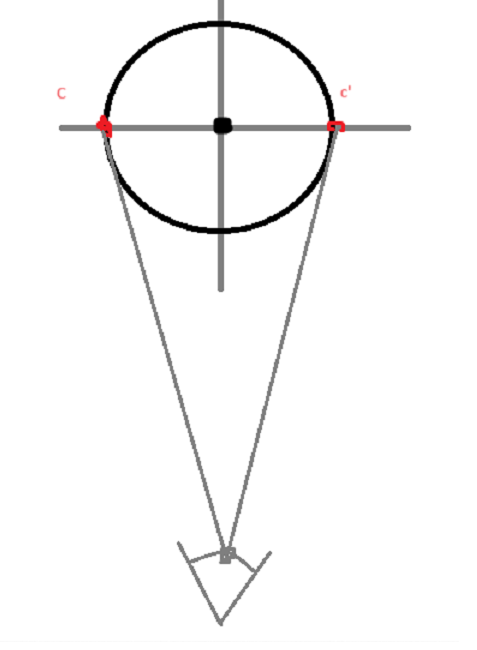
\includegraphics[scale = 0.6]{images/schema 3.png} \\
\emph{\textbf{Figure 2.} Schéma de l'orbite d'un satellite correspondant aux approximations faites.}
\end{center}

% Parler de l'alignement plus en détails -> inclure schémas
% Parler de la méthode de calcul des distances.


\section{Expérimentations et Résultats}

\subsection{Observations}
A l'origine nous souhaitions effectuer des observations de manière régulière et suffisamment bien espacée de sorte à avoir suffisamment de données pour déterminer correctement le demi-grand axe des ellipses décrites par les orbites de chaque satellite.\break

Cependant, nous n'avons pu effectuer que quelques observations en raisons d'une météo très capricieuse couplée à un lot de soucis techniques au niveau de la coupole astronomique et de délais trop courts pour compenser les caprices météorologiques de notre planète. \\
De plus ces observations n'ont pas été effectuées à des intervalles réguliers, c'est-à-dire que nous n'avons pu observer qu'aux dates suivantes: Le 25 Septembre 2023, les 3,6,7 et 10 Octobre. Sur la période de Novembre nous n'avons pu effectuer d'observations pour les raisons évoquées précédemment. Toutefois, si la durée d'un mois d'observation peut sembler courte, elle est justifiée car une durée plus longue d'observation demande de prendre en compte le déplacement de la Terre par rapport à Jupiter de façon plus poussée que ce que l'on a fait, ce qui va au delà de notre objectif de modélisation ici (pour plus de détails voir \textbf{[5]}).

\begin{center}
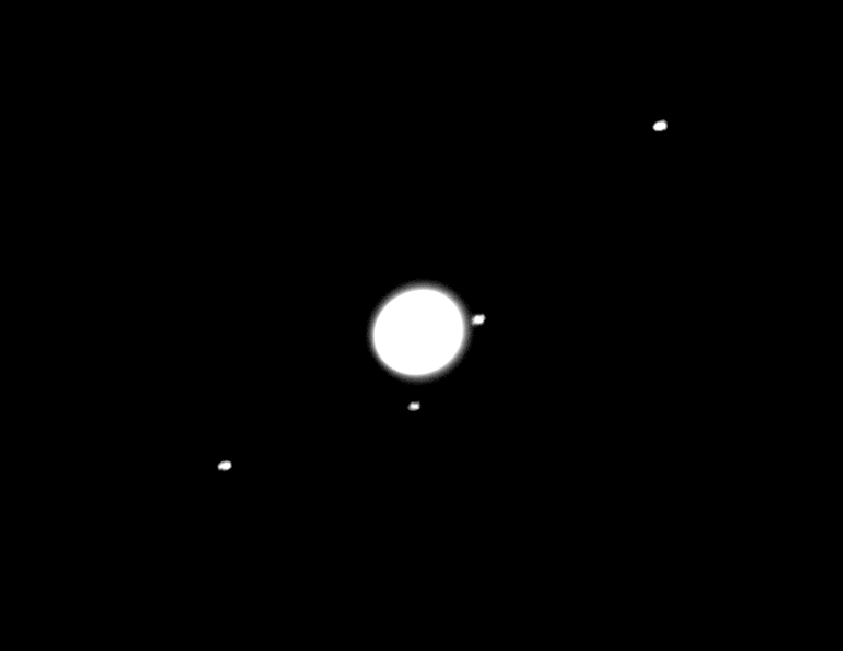
\includegraphics[scale = 0.3]{images/Exemple d'observation.PNG}\\
\emph{{\textbf{Figure 3.} Image tirée de l'observation du 25 Septembre 2023 - Temps d'exposition : 300 ms}}
\end{center}

On retrouve ci-dessus l'une des images obtenues lors de la première observation de Jupiter et de ses lunes. On observe de gauche à droite: \textit{Ganymède}, \textit{Europe}, \textit{Callisto} et \textit{Io}. Les séries possèdent les caractéristiques suivantes: \\

\begin{center}
        \begin{tabular}{|c|c|c|}
        \hline
           Date & Nombre d'images & Temps d'exposition   \\
        \hline
           25-09 & 20 & 300 ms \\
        \hline
            03-10 & 20 & 300 ms  \\
        \hline
            06-10 & 30 & 300 ms  \\
        \hline 
            07-10 & 50 & 300 ms \\
        \hline
            10-10 & 30 & 300 ms \\
        \hline
        \end{tabular}
\end{center}

        La différence du nombre d'images par prises s'explique par la prise en main du matériel et le fait que l'observateur n'était pas toujours le même. De plus nous avons dit dans la section \textbf{Matériel \& Méthodes} que les images ont été prises avec un temps d'exposition de \textit{300 ms} correspondant à une durée optimale. On place ci-dessous deux exemples d'images sous-exposées et sur-exposées pour illustrer notre propos.

\begin{center}
    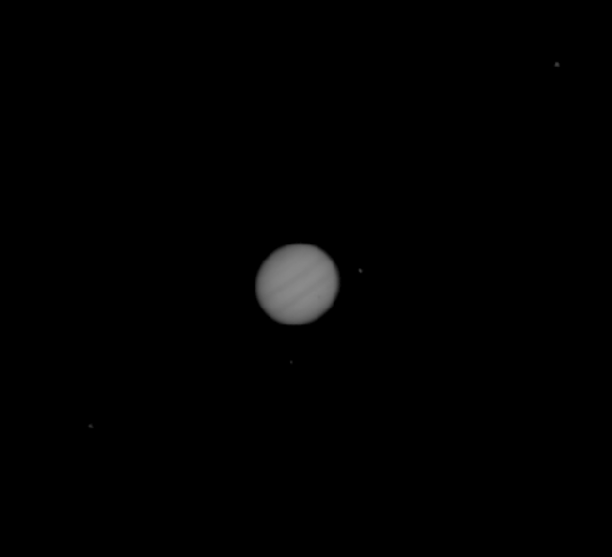
\includegraphics[scale = 0.5]{images/exemple sousexp.png} \\
    \emph{\textbf{Figure 4.} Image tirée de l'observation du 25 Septembre 2023 - Temps d'exposition : 20 ms} \break

    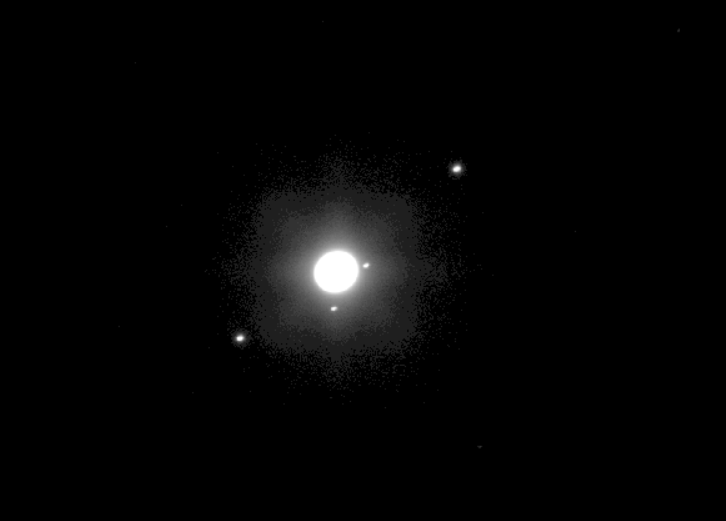
\includegraphics[scale = 0.5]{images/exemple surexp.png} \\
    \emph{\textbf{Figure 5.} Image tirée de l'observation du 25 Septembre 2023 - Temps d'exposition : 1 s} 
\end{center}

On voit bien sur le Figure 4 les bandes de Jupiter mais on distingue à peine deux des lunes et on ne voit pas du tout les deux autres. À l'inverse, sur la Figure 5, on observe parfaitement les quatre satellites mais Jupiter est clairement sur-exposée, ce qui ne permet pas une bonne exploitation de l'image.\\

À chaque fois que l'on fait une série d'observations, il est important de réaliser ce qu'on appelle les "darks" et les "flats" afin de réduire le bruit sur l'image finale.
Les darks sont une série d'images prises dans les mêmes conditions que nos images "brutes" (celles sur lesquelles Jupiter apparaît), mais lors desquelles on a mis le cache de la lunette. Cela permet de réaliser une carte thermique du capteur, pour soustraire à notre image brute les défauts dûs à la chaleur de la caméra [7]. 
Les flats quand à eux permette de corriger la présence de poussière à l'image et le phénomène de vignetage (l'assombrissement naturel des bords de l'image). Ils sont réalisés en plaçant devant la lunette une source de lumière blanche uniforme. Dans notre cas, n'étant pas présents physiquement dans la coupole et ne possédant pas de boîtier conçu pour les flats, nous avons simplement ouvert la coupole pour y faire rentrer la lumière du jour, puis visé l'intérieur de la coupole avec la lunette afin d'obtenir le résultat escompté.
Il faut également penser à réaliser des darks ayant le même temps d'exposition que les flats.

% Ajouter tout ce qu'on peut dire d'autre sur les observations 


\subsection{Analyse des Images et Résultats}
% pseudo-code des fonctions essentielles

Le traitement, l'analyse et l'exploitation des images ont constitué l'essentiel de notre travail et ont été réalisés avec le langage de programmation Python. Il a donc fallu coder un grand nombre de fonctions qui forment une chaîne, de la récupération des images brutes jusqu'au calcul de la masse de Jupiter. Nous détaillons dans cette partie le raisonnement global puis le mécanisme derrière les principales fonctions. \\

Nous préparons d'abord les images brutes en extrayant des fichiers FITS les matrices leur correspondant (chaque élément de la matrice correspondant à la valeur d'un pixel), puis en utilisant les darks et les flats dont nous avons discuté l'utilité plus haut. Nous moyennons d'abord l'ensemble des flats pour une série puis nous utilisons la formule suivante sur chacune des images de la série: \\

\begin{equation}
    I = \frac{image - dark1}{flat_{moy} - dark2 }
\end{equation}

Nous récupérons ainsi une liste d'images pré-traitées. \\
Une fois les images préparées avec les flats et les darks, on cherche à obtenir une seule image par série d'observation et qu'elle reflète au mieux la réalité. Pour cela on utilise les trois procédures successives et complémentaires évoquées au 3.3.2 \\

Détaillons la procédure pour une seule série : \\
Nous souhaitons d'abord obtenir les coordonnées de Jupiter afin de pouvoir la décaler au centre afin d'aligner les différentes images. Afin d'optimiser le temps de calcul nécessaire aux opérations, nous rognons l'image originale à une taille de \textit{1570}x\textit{1570} pixels au lieu de \textit{4656}x\textit{3520} pixels, nous aurions pu réduire plus mais pour des raisons de praticité nous gardons cette taille là, commune à l'ensemble de nos séries puisque l'on a déterminé empiriquement que c'était la seule zone pour laquelle nous ne risquions pas de rogner une ou plusieurs lunes de l'image, ce qui serait évidemment problématique. Pour calculer nos coordonnées, nous appliquons comme mentionné en 3.2.2 une fonction gaussienne pour une image donnée sur l'ensemble des valeurs des pixels de la zone donnée. \\

Il est important de noter que cela n'est efficace que parce que l'image est en niveaux de gris. Pour une efficacité optimale nous créons ce que l'on appelle un masque, qui va restreindre l'endroit de l'image sur laquelle nous appliquons la gaussienne. Une fois celle-ci créée, nous lui appliquons un ajustement gaussien à l'aide de la bibliothèque \emph{scipy}, ce qui nous permet de récupérer les coordonnées du pixel de plus forte amplitude sur l'image. Ensuite nous appliquons cela à l'ensemble de la série. \\

On ré-aligne ensuite l'ensemble des images de la série autour de Jupiter que l'on place au centre de l'image afin de pouvoir suivre de plus simplement l'évolution des lunes relativement à Jupiter au fil du temps et des observations. Nous avons obtenu l'ensemble des coordonnées de Jupiter pour chaque image de la série, il  nous reste donc à calculer l'écart nécessaire entre le centre et l'actuelle position de Jupiter afin de recentrer l'image sur elle. Nous calculons le centre via la formule $(x_0,y_0) = (\frac{n_{pix}}{2} , \frac{n_{pix}}{2})$ où $n_{pix} = 1570$, on calcule ensuite les écarts nécessaires via $(dx,dy) = (x-x_0 ,y-y_0)$ où $(x,y)$ sont les coordonnées actuelles de Jupiter.\\

Récapitulons : nous avons récupéré les coordonnées de Jupiter et procédé à un ré-alignement. On calcule alors la médiane de la série ré-alignée et nous obtenons ce type d'images: 

\begin{center}
    % Inclure image après alignement
    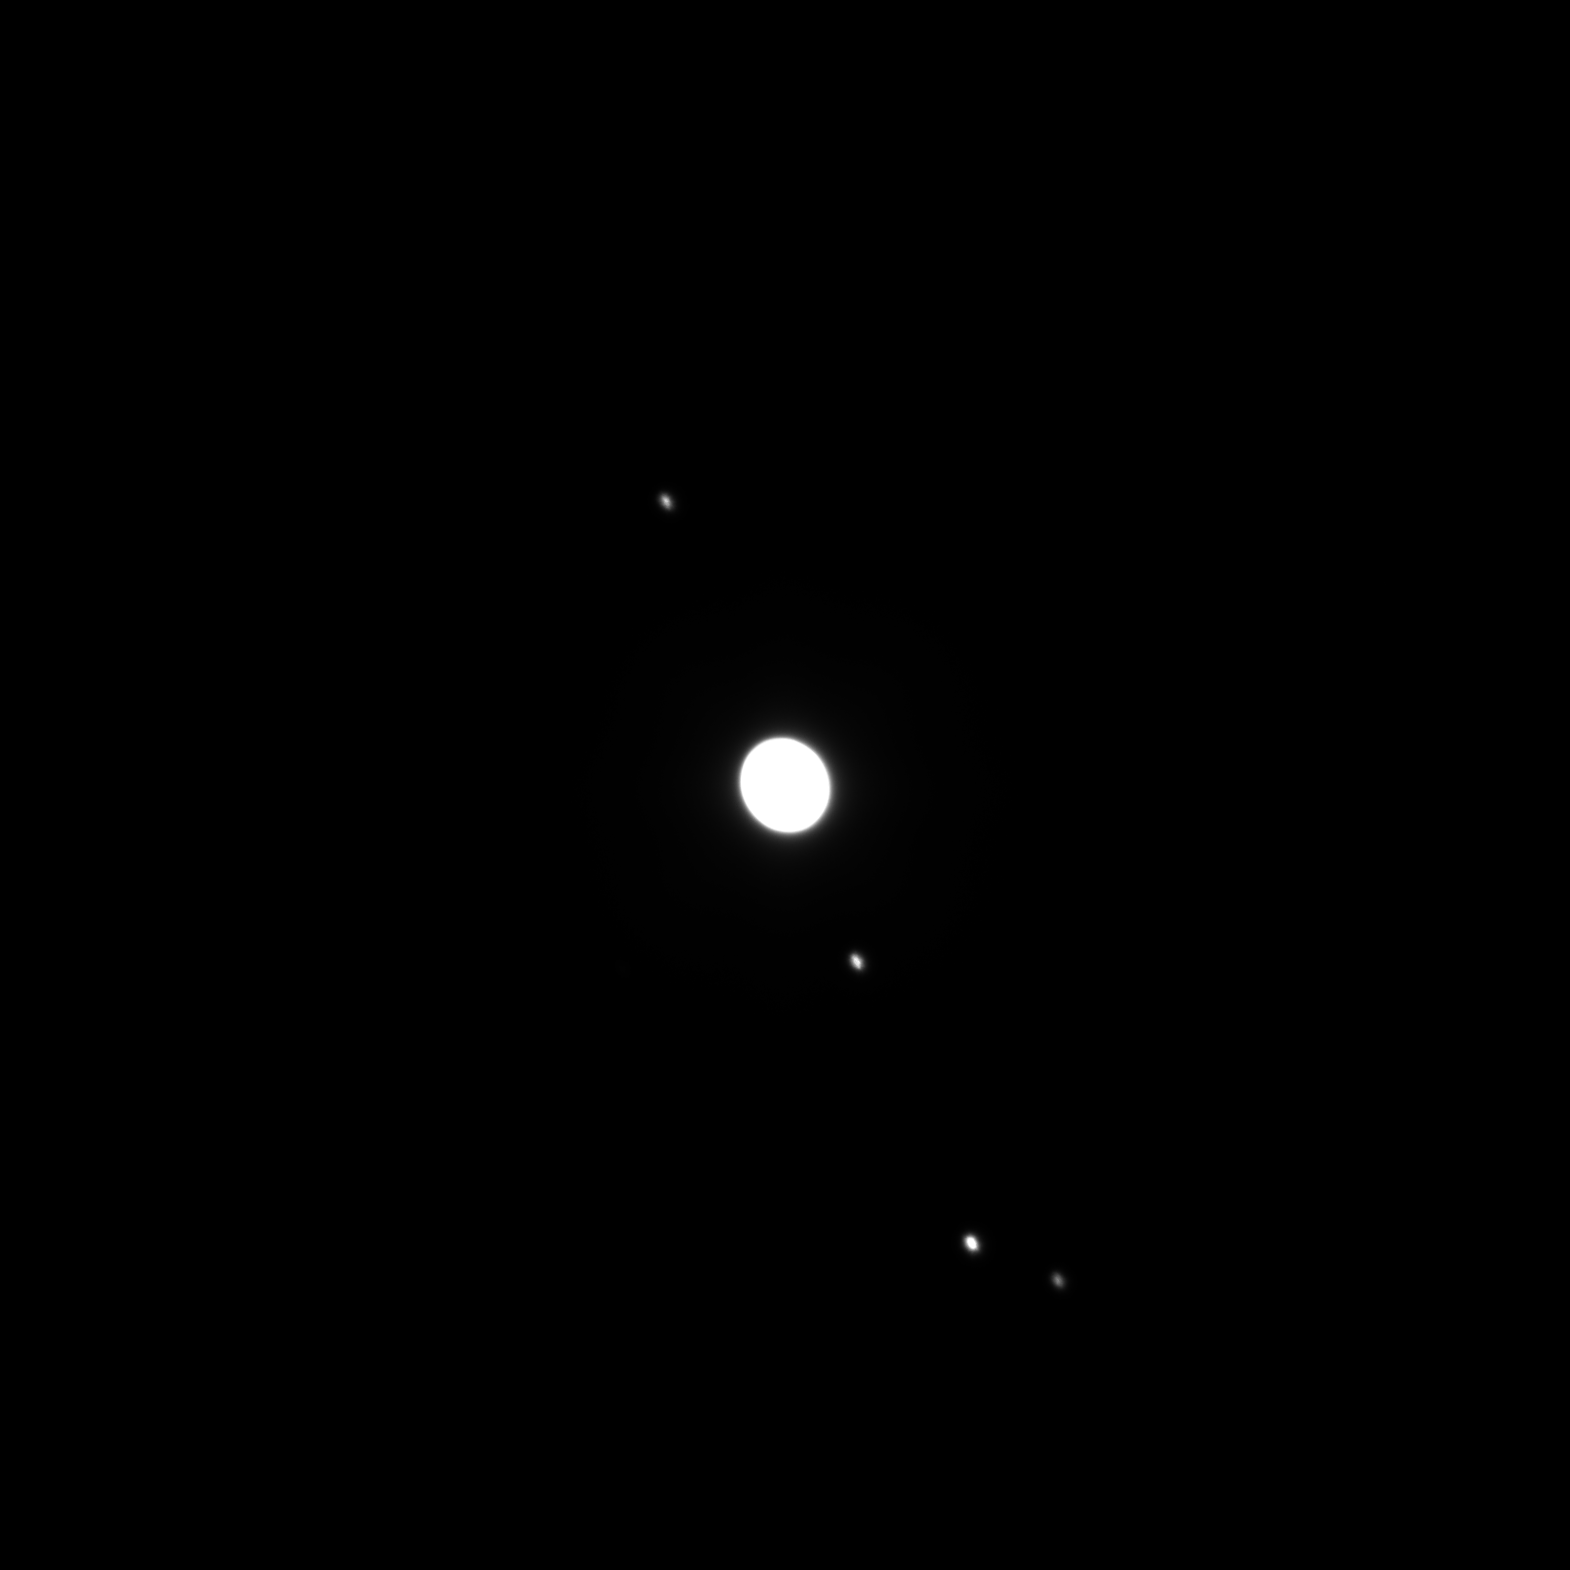
\includegraphics[scale = 0.22]{images/apres_realignement.png}
    \emph{\textbf{Figure 6.} Image obtenue après ré-alignement de la série du 10 Octobre 2023}
\end{center}

On cherche maintenant à déterminer les coordonnées de chacune des lunes. À l'origine, nous voulions utiliser une gaussienne sur les lunes de la même manière que pour Jupiter une fois la série complètement traitée, c'est-à-dire une fois les images ré-alignées et superposées. Seulement, nous nous sommes rendus compte qu'une fois le ré-alignement fait, cela faisait disparaître de l'image l'une des quatre lunes sur une série, nous empêchant par conséquent d'obtenir ses coordonnées. En effet l'écart entre Jupiter et la lune était très important, le déplacement au centre de l'image l'a donc fait sortir du cadre de l'image comme suit:

\begin{center}
    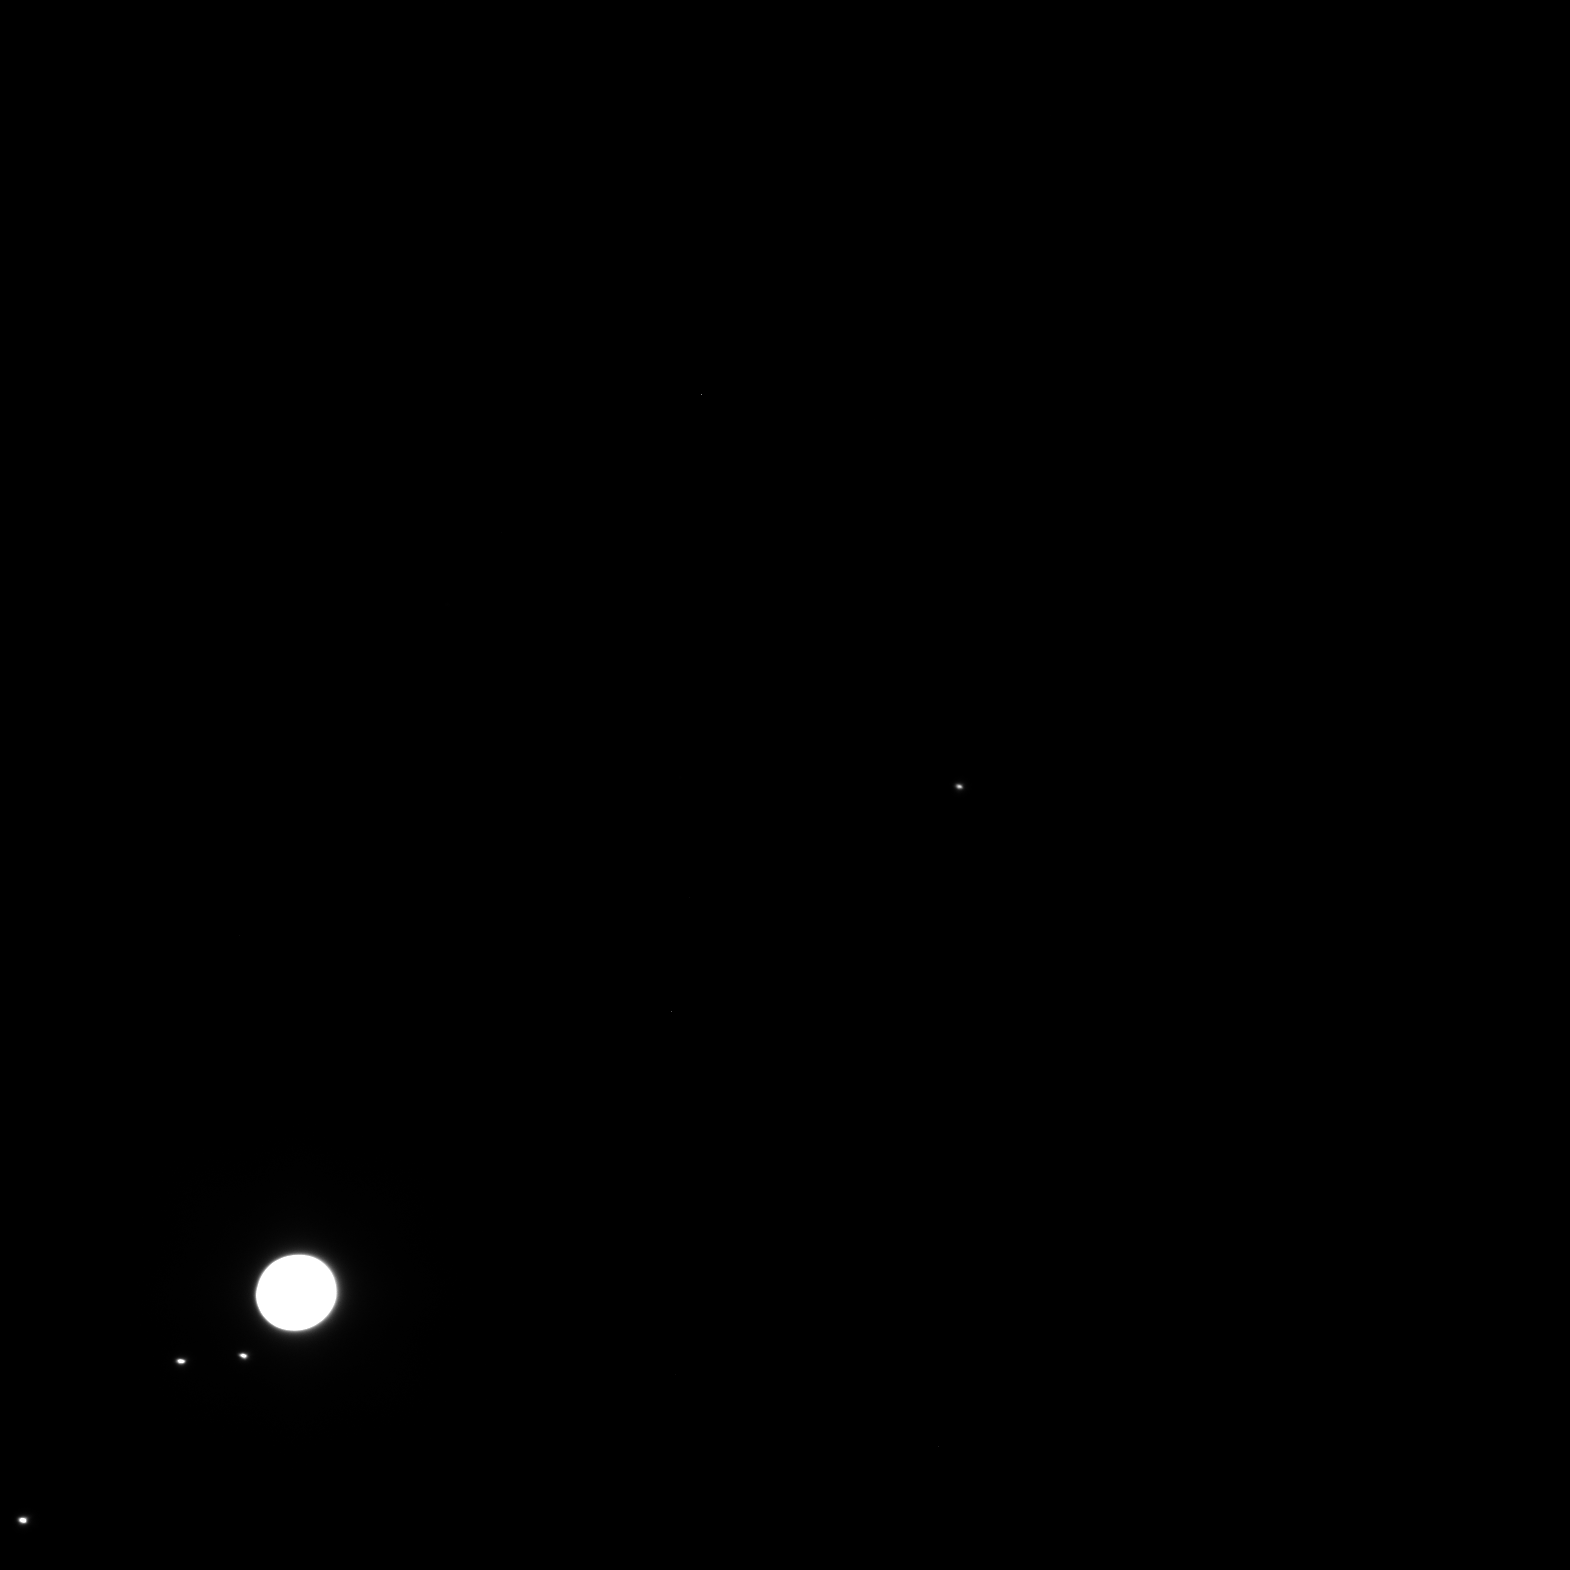
\includegraphics[scale = 0.2]{images/avant_realignement.png} \\
    \emph{\textbf{Figure 7.} Avant ré-alignement}
\end{center}

On aperçoit sur la figure 7 quatre lunes sur l'image d'origine, trois en bas à gauche de Jupiter et la troisième au milieu de l'image. \\

\begin{center}
    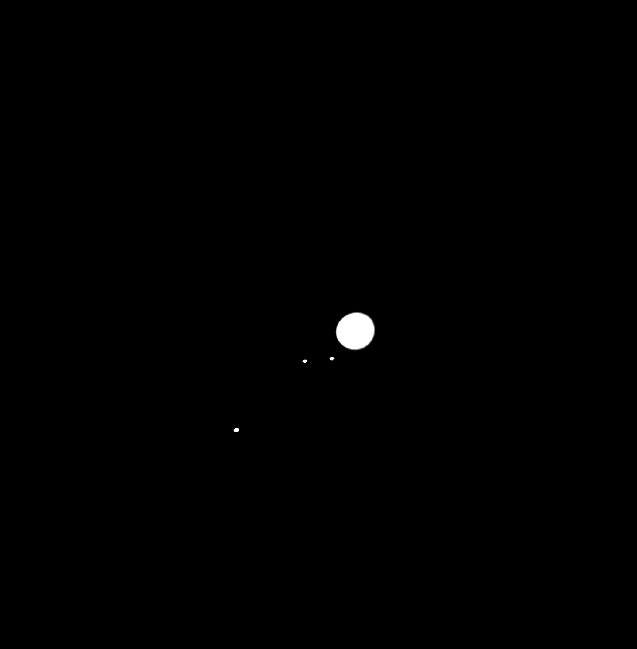
\includegraphics[scale = 0.5]{images/apres_realignement_06.png} \\
    \emph{\textbf{Figure 8.} Après ré-alignement}
\end{center}

Sur la figure 8 on ne distingue plus que trois lunes au lieu de 4.\\
Nous procédons alors d'une autre manière. Lorsque nous ré-alignons chaque image de la série, nous stockons dans un tableau les écarts $dx$ et $dy$ associés aux coordonnées $x,y$ que nous renvoyons lors de l'appel à la fonction \textit{réaligne\_serie}. Ensuite le décalage des corps observés entre chaque image étant extrêmement petit, on peut choisir arbitrairement la première image de la série afin de calculer avec la méthode gaussienne les coordonnées d'origine de chacune des lunes. On calcule ensuite la position après-alignement de chaque astre en y ajoutant le décalage calculé précédemment. Il n'est donc plus nécessaire d'avoir les astres sur l'image après alignement afin de calculer leurs coordonnées.

Une fois les coordonnées de Jupiter et des lunes acquises et stockées dans une liste, on souhaite connaître la distance séparant chaque lune de Jupiter. Nous avions tout d'abord songé à utiliser la distance euclidienne, mais cela imposait des valeurs positive par définition. Or, sachant que les orbites apparentes des lunes devraient être placées sur un sinus, il était impensable de ne pas avoir des distances algébriques.
Pour remédier à cela, nous avons commencé par centrer les coordonnées autour de Jupiter (qui devient ainsi l'origine de notre repère), puis nous avons effectué une régression linéaire (passant obligatoirement par Jupiter) afin d'obtenir une approximation du plan sur lequel évoluent les satellites galiléens. On projette ensuite les positions des différentes lunes sur cet axe, et il est maintenant aisé de récupérer dans une nouvelle liste les distances algébriques entre chaque lune et Jupiter.

\begin{center}
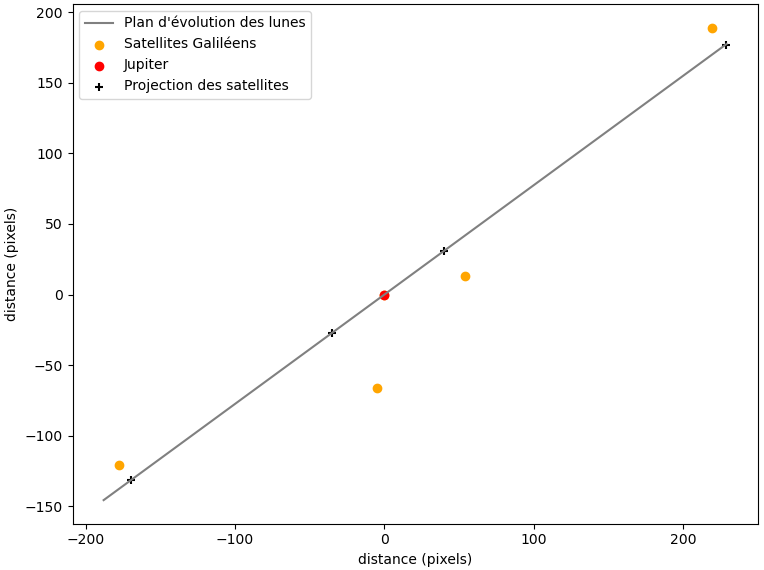
\includegraphics[scale = 0.56]{images/projection.PNG}\\
\emph{{\textbf{Figure 8.} Projection de la position des lunes pour l'observation du 25 Septembre 2023}}
\end{center}

Après avoir lancé ce programme pour chaque série (donc pour chaque observation), on obtient la position relative des quatre lunes par rapport à Jupiter et ce pour nos 5 dates d'observation. 
Dans un soucis de précision nous utiliserons comme échelle de temps le nombre de minutes écoulées depuis le 26/10 à 00h00, premier jour de nos observations.

\begin{center}
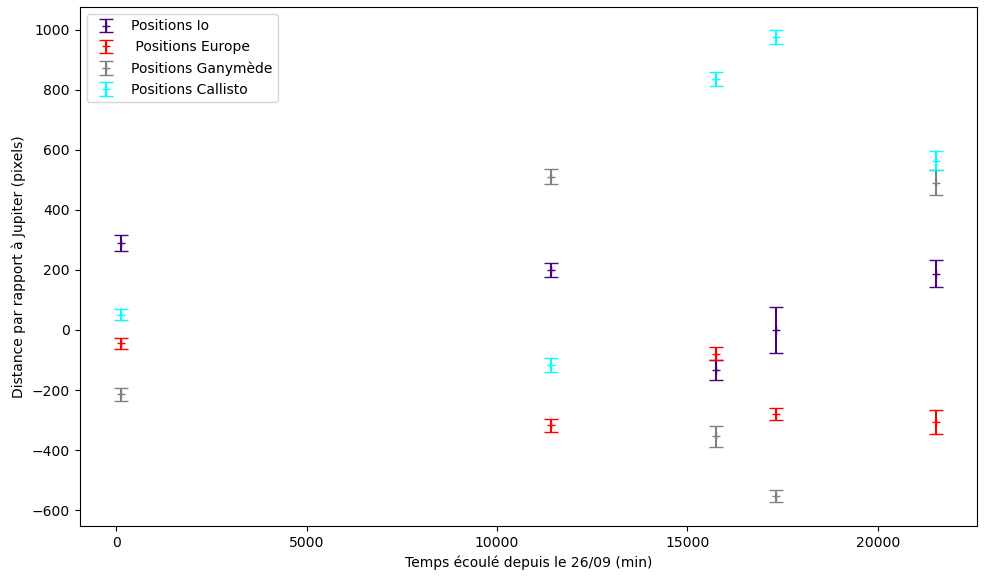
\includegraphics[scale = 0.435]{images/positions.PNG}\\
\emph{{\textbf{Figure 9.} Positions relatives des lunes par rapport à Jupiter pour l'ensemble de nos observations}}
\end{center}

On remarque que l'incertitude sur la position de Io est particulièrement importante dans la 4ème série. Cela s'explique aisément par le fait que ce soir là, au moment de prendre nos images, Io était en transit devant Jupiter ! Notre image n'ayant pas la résolution ni le temps d'exposition suffisants pour distinguer Io de Jupiter, l'incertitude sur la position de la première n'est autre que le diamètre de la seconde. \\
On souhaite désormais simuler une trajectoire orbitale qui convienne pour chacune des lunes. Vues depuis la Terre, les lunes de Jupiter paraissent effectuer un mouvement périodique autour de leur planète. Nous choisissons donc un sinus pour représenter la trajectoire. La période de chacune des lunes étant supposée connue, on la rentre dans notre programme afin d'obtenir des paramètres initiaux vraisemblables. Un ajustement sinusoïdal réalisé avec python nous donne la pulsation, l'amplitude et la phase ajustées, qu'il nous suffit ensuite de tracer. On récupère également l'incertitude sur l'amplitude de chacun des sinus, qui nous servira par la suite.
\begin{center}
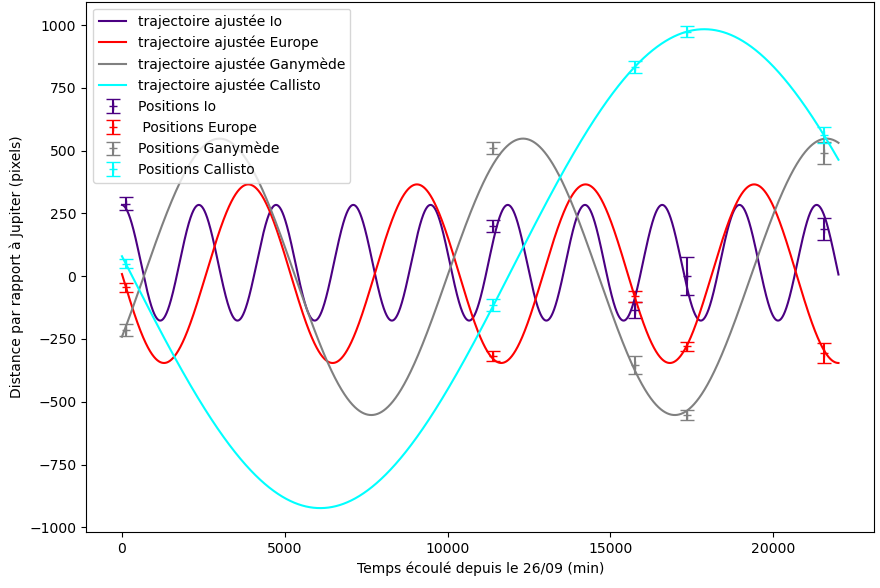
\includegraphics[scale = 0.5]{images/trajectoires.PNG}\\
\emph{{\textbf{Figure 10.} Trajectoires estimées pour les 4 satellites galiléens}}
\end{center}
Visuellement, on constate que pour Callisto et Europe les trajectoires ajustées correspondent parfaitement aux observations.
Pour Ganymède la courbe ajustée ne passe que par trois points d'observation et seulement deux pour Io, dont celui possédant une barre d'incertitude importante. On s'attend alors à avoir un demi-grand axe plus éloigné de la vérité pour Io et Ganymède que pour Callisto.\\

Cette étape ne servait qu'à confirmer visuellement que notre trajectoire simulée était au moins probable, à défaut d'être exacte. On peut enfin récupérer le demi-grand axe de chacun des satellites, qui correspond à la distance maximale entre Jupiter et le satellite. Dans notre programme il s'agit simplement de l'amplitude des sinus ajustés.\\
On utilise à nouveau la formule (4) en sens inverse cette fois pour convertir l'amplitude en radians, puis un peu de trigonométrie  s'appuyant sur la distance moyenne entre la Terre et Jupiter durant la quinzaine d'observation pour déterminer le rayon satellite/Jupiter en km avec ses incertitudes. Ces incertitudes proviennent principalement de l'ajustement des sinus effectué plus tôt, mais aussi de la distance variable entre la Terre et Jupiter. Bien que pour une date donnée elle soit connue avec grande précision, nos observations se sont étalées sur une quinzaine de jours, entraînant une modification progressive de cette distance. Afin d'en rendre compte nous avons ajouté à la distance moyenne une incertitude correspondant à la moitié de la plage de distances possibles.\\

On possède désormais les deux valeurs qui nous intéressent pour démontrer la troisième loi de Kepler : 
\begin{itemize}
    \item la période \emph{T} de chacune des lunes (supposée connue depuis le début).
    \item le demi-grand axe \emph{a} (approximé par un rayon \emph{r} constant) de chacune des lunes.
\end{itemize}
On trace alors $T^2/a^3$ et l'on fait une dernière régression linéaire pondérée sur nos quatre points. La pente de cette régression nous donne la valeur de la constante de proportionnalité que l'on retrouve dans la troisième loi de Kepler.  
\begin{center}
    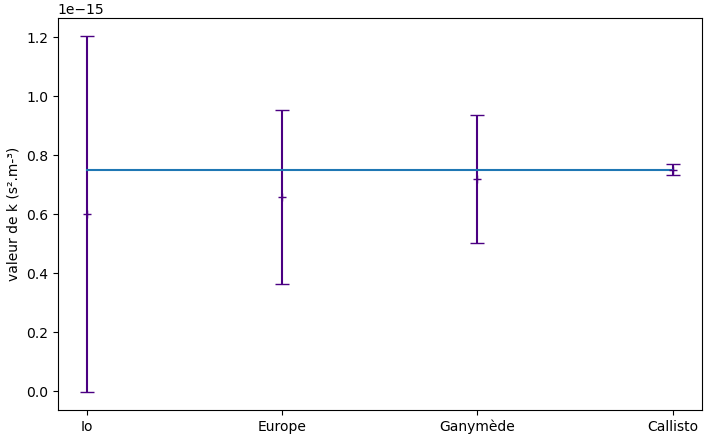
\includegraphics[scale = 0.62]{images/kepler.PNG}\\  
    \emph{{\textbf{Figure 11.} Valeurs de $T^2/a^3$}}
\end{center}
Remarquons la forme particulière des incertitudes sur la valeur de $T^2/a^3$ : plus la lune est éloignée, plus les incertitudes sont faibles. Cela est vrai depuis la modélisation par des sinus et s'explique en réalité assez aisément. Au cours de nos différentes observations, pour une lune plus éloignée qu'une autre, on observe des positions plus "proches" les unes des autres proportionnellement parlant, en vertu de la deuxième loi de Kepler. L'incertitude sur l'amplitude du sinus modélisant la trajectoire de Callisto est donc bien plus faible que celle sur l'amplitude de Io.\\
 On obtient la valeur de k suivante :
 
 \begin{equation}
     k = 7,5.10^{-16} \pm 6,6.10^{-17} s^{2}.m^{-3}
 \end{equation}\\
 L'incertitude sur k provient de la moyenne des écarts entre les points $T^2/a^3$ et la courbe de la régression linéaire.   
 Nous avons ainsi démontré qu'il existe bel et bien une relation de proportionnalité entre le carré de la période des lunes de Jupiter et le cube de leur demi-grand axe.\\

 On cherche finalement à répondre à la demande suivante : "Déterminer la masse de Jupiter à partir de la 3ème loi de Kepler."\\
 Pour cela on utilise la forme newtonnienne de la loi des périodes (3), démontrée en annexe. 
 Alors :
 \begin{equation}
     M_{Jupiter} = \frac{4\pi^2}{kG}  
 \end{equation}
Où G la constante gravitationnelle que l'on prendra équivalente à $ G \approx 1,674.10^{-11} \; m^3.kg^{-1}.s^{-2}$ \\
On obtient : 
 \begin{equation}
    M_{Jupiter} = 3,14.10^{27} \pm 2,76.10^{26} \; kg  
 \end{equation}
 Or la masse réelle de Jupiter est :
\begin{equation}
    M_{attendue} = 1,898.10^{27} \; kg
\end{equation}
On peut alors calculer l'écart normalisé (parfois aussi appelé Z-score) entre les valeurs obtenues et attendues pour la masse de Jupiter [8].
\begin{equation}
    \eta = \frac{|M_{Jupiter}-M_{attendue}|}{u(M_{Jupiter})} = 4.5
\end{equation}
Cet écart normalisé est assez important. Par exemple pour une distribution gaussienne des résultats, $\eta = 2 $ signifierait que les résultats sont compatibles avec une certitude de 95\%. Dans notre cas il y a plutôt incompatibilité entre la mesure et la valeur théorique, ce que l'on cherche à expliquer. 

\section{Conclusion}

On obtient une masse de Jupiter qui est du bon ordre de grandeur ($10^{27} kg$), toutefois nos incertitudes sont sous-estimées car elles ne permettent pas de rendre compte de la masse réelle de la planète.
Nous avons émis plusieurs hypothèses expliquant cette difficulté : 
\begin{itemize}
    \item L'approximation faite à la Figure 8 qui consiste à passer d'un problème en 2D à un problème en 1D (physiquement, cela revient à supposer que l'on observe Jupiter et ses lunes dans le plan d'évolution de ces dernière) induit forcément des incertitudes quand à la distance lune/Jupiter, que nous n'avons pas su prendre en compte. Il aurait peut être fallu trouver un moyen de modéliser différemment les orbites des lunes, peut être en définissant notre propre distance.
    \item La conversion entre le nombre de pixels sur nos images et le nombre de km dans la réalité avec la formule (7) peut rapidement conduire à des erreurs de mesure. Comme les lunes ne font qu'une vingtaine de pixels de diamètre, une erreur d'estimation de leur taille a des conséquences importantes dans notre calcul.
    \item Nous aurions voulu pouvoir observer de façon plus fréquente lors des 15j d'observations de notre projet. Cela aurait permis de mieux modéliser la trajectoire des lunes les plus proches de Jupiter : Io et Europe.
\end{itemize}

Malgré les différentes difficultés rencontrées, nous avons su obtenir des résultats relativement probants que nous pourrions encore améliorer en prenant en compte l'ensemble des approximations faites au cours de la modélisation et de l'expérience.
%\begin{flushleft}
%        \begin{tabular}{|c|c|c|c|}
%        \hline
%           Lune & théorique (km) & expérimentale (km) & Écart (\%)   \\
%        \hline
%           I & 421800 & 338741 & 24 \\
%        \hline
%            E & 671100 & 522839 & 28 \\
 %       \hline
    %        G & 1070400 & 810032  & 32\\
 %       \hline 
 %           C & 1882700 & 1403565 & 34 \\
%        \hline
  %      \end{tabular}
%\end{flushleft}

% image résultante
% Exemple de coordonnées obtenues
% Plot de l'évolution des distances et commentaires qui vont avec


%--------------------------------------------------%
%\begin{acknowledgements}
%\end{acknowledgements}

% WARNING
%-------------------------------------------------------------------
% Please note that we have included the references to the file aa.dem in
% order to compile it, but we ask you to:
%
% - use BibTeX with the regular commands:
%   \bibliographystyle{aa} % style aa.bst
%   \bibliography{Yourfile} % your references Yourfile.bib
%
% - join the .bib files when you upload your source files
%-------------------------------------------------------------------
\begin{flushleft}

\begin{thebibliography}

  \item \textbf{[1]} \url{https://fr.wikipedia.org/wiki/Lois_de_Kepler} (le 3 octobre 2023),  Wikipedia Lois de Kepler\\
  \item \textbf{[2]} \url{https://fr.wikipedia.org/wiki/Satellites_galil%C3%A9ens} (le 3 octobre 2023),Wikipedia, Satellites Galiléens\\
  \item \textbf{[3]}  \url{https://fr.wikipedia.org/wiki/Vitesse_ar%C3%A9olaire} (le 18 octobre 2023) Wikipedia, Vitesse aréolaire \\
  \item \textbf{[4]} \url{http://chaours.rv.pagesperso-orange.fr/Astro/telescope.htm} (le 13 octobre 2023) Chaoursrv Astronomie\ Télescope\\
  \item \textbf{[5]} Bridges, R. Fitting Orbits to Jupiter’s Moons with a Spreadsheet. Phys. Educ. 1995, 30 (5), 272–276. \url{https://doi.org/10.1088/0031-9120/30/5/003}.
  \item \textbf{[6]} Lyra, W. A Historical Method Approach to Teaching Kepler’s 2nd Law. 2020. \url{https://doi.org/10.48550/ARXIV.2011.13386}.
  \item \textbf{[7]} \url{https://www.blue-sunset.fr/astrophotographie-dark-offset-flat-explication-description-realisation-comment} Astrophotographie: Dark – Flat – Offset (consulté le 25 novembre 2023).
  \item \textbf{[8]} \url{https://fr.wikipedia.org/wiki/Jupiter_(plan%C3%A8te)} (le 1er décembre 2023), Wikipedia Jupiter
    }
    

 
\end{thebibliography}

\textit{\textbf{Répartition du travail:}} \\
- Justin : Grande majorité du programme informatique de traitement, moitié du rapport, quelques observations. \\
- Antonin : Partie du programme informatique, moitié du rapport, quasi-totalité des observations.


\end{flushleft}

\newpage
% ================= ANNEXE ==================== %
\section{Annexe}

Dans cette partie nous allons démontrer mathématiquement les trois lois de Kepler: Loi des Orbites, des Aires, des Périodes pour une lune L orbitant autour de Jupiter (J).  Pour cela nous nous plaçons en repère cylindrique centré en $J$ : $\left(J, \vv{u_r}, \vv{u_\theta}, \vv{u_z}\right)$ et nous introduisons les grandeurs suivantes: 

\begin{itemize}
    \item $m_J$ la masse de Jupiter \\
    \item $m_L$ la masse de la lune orbitant autour de Jupiter \\ 
    \item $r$ la norme du vecteur $\vv{JL}$ \\
    \item $\theta$ l'angle du vecteur $\vv{JL}$ par rapport à l'axe $\left(Jx\right)$ orienté dans le sens positif. ( voir \emph{Figure 2} ) \\
    \item $G$ la constante de gravitation universelle. \\
    \item $p$ le paramètre de l'ellipse avec $\left[p\right] = 1 $ \\
    \item $e$ l'excentricité de l'ellipse avec $\left[e\right] = 1 $ \\
    \item $\vv{v}$ la vitesse de la lune L par rapport à Jupiter, de norme $v = \| \vv{v} \|$ \\
    \item $\vv{\sigma}_J$ le moment cinétique de $L$ autour du point fixe $J$ \\
    \item $a$ le demi-grand axe de l'ellipse \\
    \item $b$ le demi-petit axe de l'ellipse  \\
    \item $C$ la constante des aires \\
\end{itemize}


\subsection{Démonstration des Lois de Kepler}

\subsubsection{Première loi : Loi des Orbites }

Démontrons que la trajectoire de L autour de Jupiter décrit une trajectoire elliptique de rayon $r = \frac{p}{1+ecos(\theta)}$ et $C^2 =Gm_Jp $ où $C$ est la constante des aires, $G$ la constante de gravitation universelle, $m_J$ la masse de Jupiter et $p$ le paramètre de l'ellipse. \\


On se place dans un repère cylindrique $(J,\vv{u_r}, \vv{u_\theta}, \vv{u_z})$
. On considère le mouvement plan dans le plan $(\vv{u_r},\vv{u_\theta}).$ ( On l'admet pour le moment, on le démontrera lors de la démonstration de la seconde loi de Kepler ). \\
On commence donc par calculer l'énergie mécanique ( $E_{tot}
$ ) de la lune L orbitant autour de Jupiter. \break

Par définition: $E_{tot} = E_c + E_p$. Or, L n'est soumise qu'à la force d'attraction gravitationnelle :
\begin{equation}
    \overrightarrow{F}_{J\rightarrow L} = -G\frac{m_Jm_L}{r^2}\vv{u_r}    
\end{equation}
qui est une force centrale. Donc conservative. D'où $\overrightarrow{F}_{J\rightarrow L}$ possède une énergie potentielle vérifiant: 

\begin{equation}
    \overrightarrow{F}_{J\rightarrow L}= -\overrightarrow{grad}(E_p)
\end{equation}
    
\begin{flushleft}
On a, en cylindrique, pour un scalaire $X$ :
\end{flushleft}

\begin{equation}
    \overrightarrow{grad}\left( X\right) = \frac{\partial{X}}{\partial{r}}\vv{u_r} + \frac{1}{r}\frac{\partial{X}}{\partial{\theta}}\vv{u_\theta} + \frac{\partial{X}}{\partial{z}}\vv{u_z}
\end{equation}
On obtient alors : 
\begin{equation}
E_p = \frac{-Gm_jm_L}{r}
\end{equation}
Or, $E_c = \frac{1}{2} m_L v^{2}$. De plus, la vitesse s'exprime dans notre repère par $\vv{v}=\dot{r}\vv{u_r} + r\dot{\theta}\vv{u_\theta}$, on a alors:

\begin{equation}
    E_{tot} = \frac{1}{2}m_L(\dot{r}\vv{u_r} + r\dot{\theta}\vv{u_\theta})^{2} + \frac{-Gm_jm_L}{r}
\end{equation}
\begin{flushleft}
On exprime maintenant $C = r^{2}\dot{\theta} = r^{2} \frac{d\theta}{dt}$ et ainsi:

\begin{equation}
    E_{tot} = \frac{1}{2}m_L(\dot{r}\vv{u_r} + r\dot{\theta}\vv{u_\theta})^{2} + \frac{-Gm_jm_L}{r} (1) \
\end{equation}

D'où
    
\end{flushleft}
\begin{equation}
    E_{tot} = \frac{1}{2}m_L\left[ \left(\frac{dr}{dt}\right)^{2} + \frac{C^{2}}{r^{2}}\right] + \frac{-Gm_jm_L}{r}
\end{equation}

On effectue maintenant le changement de variable suivant : $\frac{dr}{dt} = \frac{dr}{d\theta}\frac{d\theta}{dt}$ \\
Puis on remplace dans (7):
\begin{equation}
    E_{tot} = \frac{1}{2}m_L\left[ \left( \frac{dr}{d\theta}\right)^{2} \left(\frac{d\theta}{dt}\right)^{2}+ \frac{C^{2}}{r^{2}}\right] + \frac{-Gm_jm_L}{r}
\end{equation}
\begin{flushleft}
On factorise ensuite (8) par $C^{2}/r^{2}$ ce qui donne:

\begin{equation}
    E_{tot} = \frac{1}{2}m_L\frac{C^{2}}{r^{2}}\left[  \frac{1}{r^{2}}\left(\frac{dr}{d\theta}\right)^{2}  + 1 \right] + \frac{-Gm_jm_L}{r}
\end{equation}
\end{flushleft}

On effectue à un nouveau un changement de variable, on pose maintenant $u = \frac{1}{r^{2}}$ $\Rightarrow \space \frac{du}{d\theta} = - \frac{1}{r^{2}}\frac{dr}{d\theta}$ et ainsi:

\begin{equation}
    E_{tot} = \frac{1}{2}m_L C^{2}\left[ \left( \frac{du}{d\theta}\right)^{2} + u^{2}\right] - uGm_jm_L 
\end{equation}

On a une expression de l'énergie mécanique de la Lune, et la force $\vv{{F}_{J}}$ est une force conservative, donc son énergie mécanique est constante. On dérive alors $E_{tot}$ selon $\theta$ et on obtient: 

\begin{equation}
    0 = \frac{1}{2}m_LC^{2}\frac{d}{d\theta}\left[ \left( \frac{du}{d\theta}\right) ^{2} + u^{2}\right] - \frac{du}{d\theta}Gm_Jm_L  
\end{equation} 

On simplifie le facteur $\frac{1}{2}$ par le facteur $2$ sortant des dérivées.

\begin{equation}
         0 = m_LC^{2}\left[ \frac{du}{d\theta}\left( \frac{d^{2}u}{{d\theta^{2}}}\right) + u\frac{du}{d\theta} \right] - \frac{du}{d\theta}Gm_Jm_L  
\end{equation}

On place ensuite $m_L\frac{du}{d\theta}$ en facteur de notre expression (12) et les deux termes étant non nuls - $ u = \frac{1}{r(\theta)}$ avec $ r \ne 0$ - on peut simplifier par ce terme pour finalement obtenir une équation différentielle linéaire en $u$ : 

\begin{equation}
    \frac{d^{2}u}{{d\theta}^{2}} + u = \frac{Gm_J}{C^{2}}
\end{equation}
\begin{flushleft}
    De solution:
    \begin{equation}
       u = Acos(\theta) + \frac{Gm_J}{C^{2}}
    \end{equation}

On obtient donc, avec $ u = \frac{1}{r}$:
\begin{equation}
    r = \frac{1}{Acos(\theta) + \frac{Gm_J}{C^{2}}}
\end{equation}
\end{flushleft}

\begin{flushleft}
    On pose alors:
    \item - $\frac{1}{p} = \frac{Gm_J}{C^{2}}$ le paramètre de l'ellipse.
    \item - $e = A$  l'excentricité de l'ellipse.\break
    
    Ce qui livre finalement:
    \begin{center}
        $r = \frac{p}{1 + ecos(\theta)}$ et $C^{2} = Gm_Jp $
    \end{center}
    
\end{flushleft}
Reste à exprimer  $p = \frac{b^2}{a} = a(1-ecos^2(theta)) $ =

%----------------------------------------------------------------------------%

\subsubsection{Deuxième loi: Loi des Aires}

 Le but de cette partie est de démontrer la seconde loi de Kepler, aussi appelée la loi des aires, qui s'énonce comme suit : L'aire balayée par la lune orbitant autour de Jupiter balaie des aires égales en des temps égaux. \break

On garde les mêmes notations que précédemment, on commence par montrer que le moment cinétique de la lune L relativement à Jupiter - i.e au point J - est constant:
    
\begin{equation}
     \vv{\sigma}_J = \vv{JL} \wedge m\vv{v} = m\vv{r} \wedge \vv{v}
\end{equation}

\begin{flushleft}
    On dérive (16): \\
    \begin{equation}
        \frac{d\vv{\sigma}_J}{dt} = m\frac{d\vv{r}}{dt} \wedge \vv{v} + m\vv{r} \wedge \vv{v} 
    \end{equation} \\
\end{flushleft} 


Or \large{ $\frac{d\vv{r}}{dt} = \vv{v}$} et \large{$\frac{d\vv{v}}{dt} = \vv{a}$}, et l'accélération $\vv{a}$ est centripède donc parallèle à $\vv{r}$. Par propriété du produit vectoriel on obtient directement: 


\begin{gather}
\vv{\sigma}_J = \vv{0}
\end{gather}


Par la même occasion, $\vv{JL}$ et $\vv{v}$ sont orthogonaux au vecteur constant $\vv{\sigma}_J$, orienté selon le vecteur $\vv{u_z}$ . Alors le mouvement est bien plan comme on l'avait supposé dans la démonstration de la première loi.\break

Maintenant le but est de relier l'aire au moment cinétique. Par définition d'un produit vectoriel:
$\| \vv{a} \wedge \vv{b} \| = absin(\alpha)$ où $\alpha$ est l'angle entre les vecteurs $\vv{a}$ et $\vv{b}$. De plus, étant donné un triangle ABC formé par les vecteurs $\vv{a},\vv{b},\vv{c}$, en notant $A_t$ l'aire du triangle ABC on a: \large{$A_t = \frac{absin(\alpha)}{2}$}. Cette propriété livre donc, pour une aire $dA_t$ balayée pendant un temps $dt$:

    \begin{equation}
       \| \vv{r} \wedge \vv{v} \| = 2 \frac{dA_t}{dt}
    \end{equation}

\begin{flushleft}
    Or $\| \vv{r} \wedge \vv{v} \| =  \frac{\|\vv{\sigma}_J\| }{m}$, en remplaçant on obtient alors:
    \begin{equation}
        \frac{\|\vv{\sigma}_J\| }{2m}=  \frac{dA_t}{dt}
    \end{equation}

    En intégrant (20) sur un intervalle temporel $[0,t]$:
    \begin{equation}
         A_t = \frac{\|\vv{\sigma}_J\| }{2m}t
    \end{equation}
\end{flushleft}

    On a donc démontré que le moment cinétique de la lune L relativement à J est constant, alors (21) livre la seconde loi de Kepler ainsi énoncée au début du paragraphe.\break

    En calculant le moment cinétique $\vv{\sigma}_J$ on obtient l'expression de la constante des aires: $C^2 = r^2\frac{d\theta}{dt}$  \break
    On démontre alors également une seconde expression de la loi des aires grâce à la constante des aires. On se place dans le triangle représenté en \emph{Figure 1}: 

    \begin{center}
        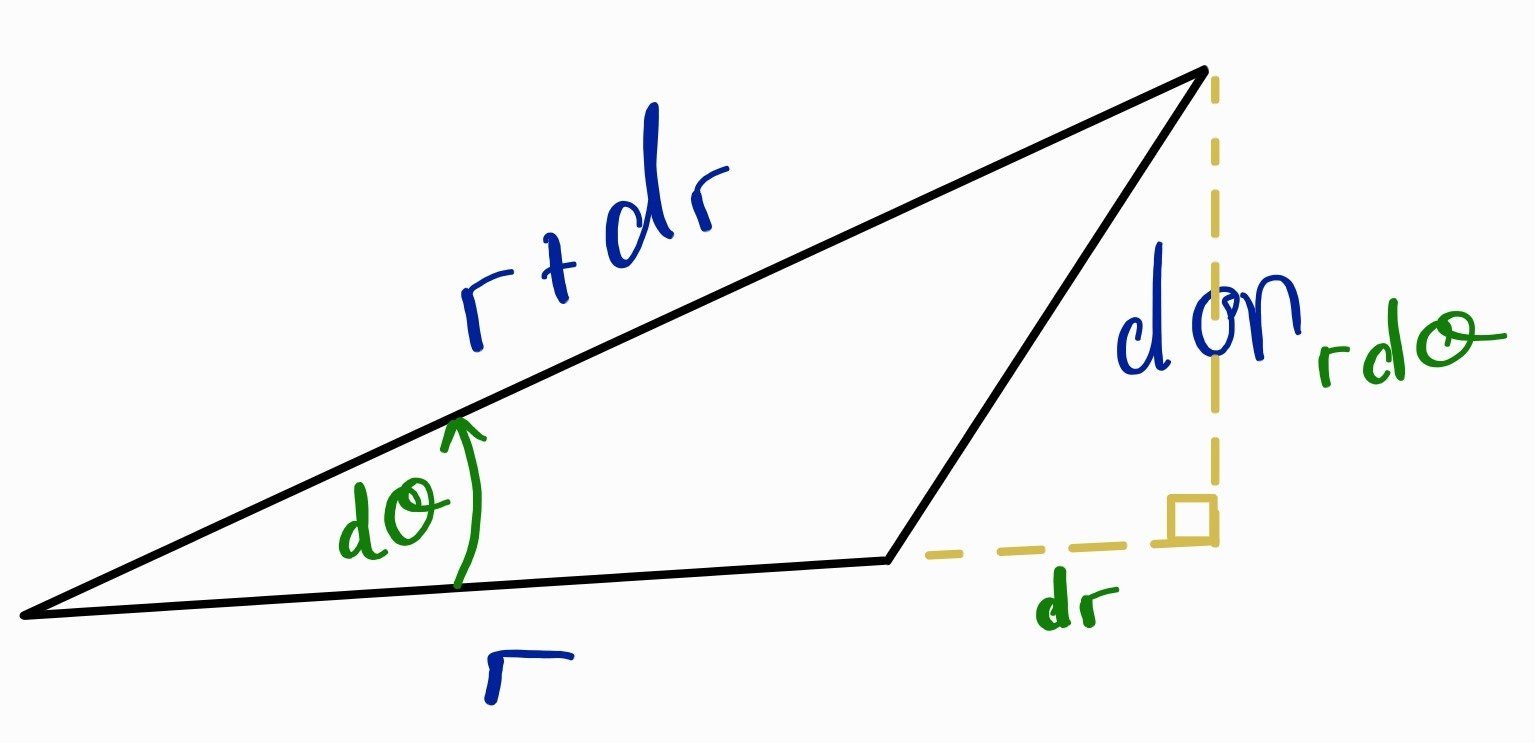
\includegraphics[scale = 0.20]{images/triangle.jpg}
        \emph{\textbf{Figure 1}. Triangle illustrant la loi des aires.}
    \end{center}
    
\begin{flushleft}
    On calcule l'aire de ce triangle et on obtient:
    \begin{equation}
        \frac{dA_t}{dt} = \frac{1}{2} r^2 \frac{d\theta}{dt} = \frac{C}{2}
    \end{equation}

    On intègre (14) sur $[0,t]$ ce qui livre:

    \begin{equation}
        A_t = \frac{C}{2}t
    \end{equation}
\end{flushleft}        

\subsubsection{Troisième loi: Loi des Périodes}


    Le but est de démontrer que le rapport suivant $\frac{T^2}{a^3}$ est une constante vérifiant: $\frac{T^2}{a^3} = \frac{4\pi^2}{Gm_J}$ 
    On utilisera pour cela les résultats démontrés par la première et la deuxième loi. \break

    On va calculer l'aire balayée par la lune L lors d'une période T de rotation autour de Jupiter dans une ellipse. \\

    \begin{center}
        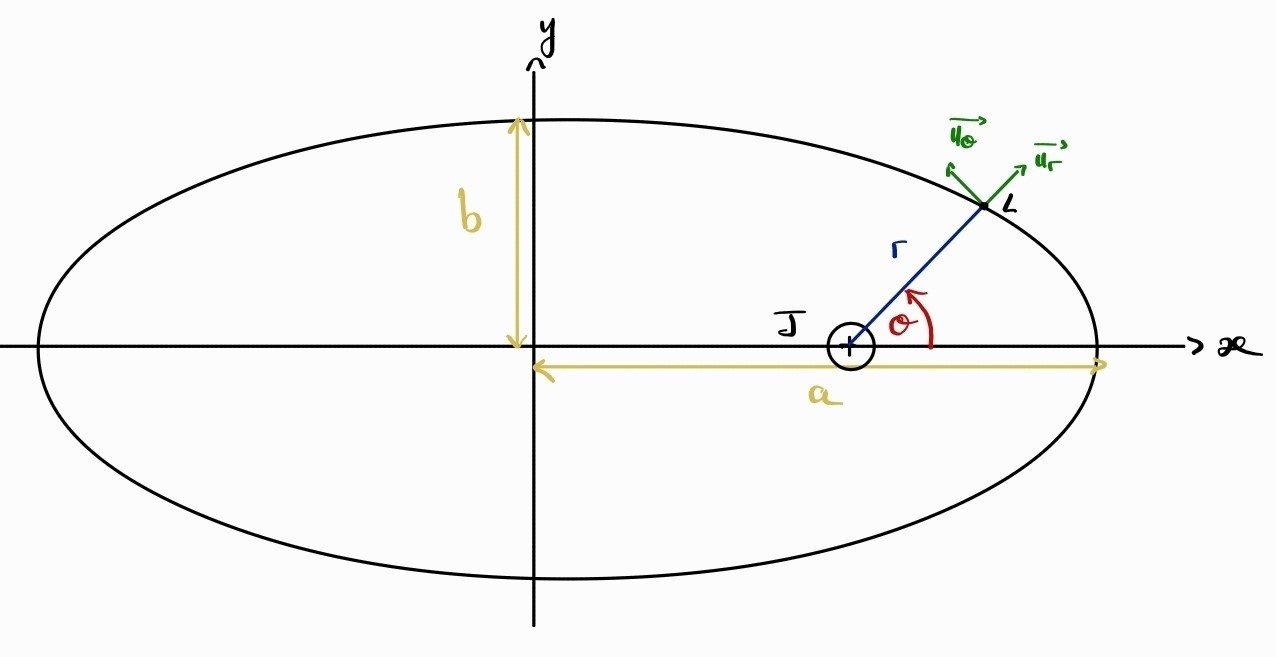
\includegraphics[scale = 0.25]{images/ellipse1.jpg}    
        \emph{\textbf{Figure 2}. Ellipse illustrant la trajectoire orbitale de la lune L autour de Jupiter}
    \end{center}
    
\begin{flushleft}
    

    La loi des aires livre alors:

    \begin{equation}
        A_T = \pi ab = \frac{C}{2}T
    \end{equation}
\end{flushleft} 

    Or la  démonstration de la première loi livre $p = \frac{b^2}{a}$ et $C^2 = Gm_Jp$, d'où, en élevant (24) au carré et en remplaçant $p$ et $C^2$ par leurs expressions:

    \begin{equation}
        \frac{T^2}{a^2} = \frac{4\pi ^2 pa}{Gm_Jp}
    \end{equation}

    On simplifie alors par $p$ dans le second membre de l'équation et on passe $a$ à gauche, ce qui livre finalement: 
    
    \begin{equation}
        \frac{T^2}{a^3} = \frac{4 \pi ^2}{Gm_J}
    \end{equation}

\end{document}
%
%%%%%%%%%%%%%%%%%%%%%%%%%%%%%%%%%%%%%%%%%%%%%%%%%%%%%%%%%%%%%%
Example below of non-structurated natbib references  
To use the v8.3 macros with this form of composition of bibliography, 
the option "bibyear" should be added to the command line 
"\documentclass[bibyear]{aa}".
%%%%%%%%%%%%%%%%%%%%%%%%%%%%%%%%%%%%%%%%%%%%%%%%%%%%%%%%%%%%%%

\begin{thebibliography}{}

  \bibitem[1966]{baker} Baker, N. 1966,
      in Stellar Evolution,
      ed.\ R. F. Stein,\& A. G. W. Cameron
      (Plenum, New York) 333

   \bibitem[1988]{balluch} Balluch, M. 1988,
      A\&A, 200, 58

   \bibitem[1980]{cox} Cox, J. P. 1980,
      Theory of Stellar Pulsation
      (Princeton University Press, Princeton) 165

   \bibitem[1969]{cox69} Cox, A. N.,\& Stewart, J. N. 1969,
      Academia Nauk, Scientific Information 15, 1

   \bibitem[1980]{mizuno} Mizuno H. 1980,
      Prog. Theor. Phys., 64, 544
   
   \bibitem[1987]{tscharnuter} Tscharnuter W. M. 1987,
      A\&A, 188, 55
  
   \bibitem[1992]{terlevich} Terlevich, R. 1992, in ASP Conf. Ser. 31, 
      Relationships between Active Galactic Nuclei and Starburst Galaxies, 
      ed. A. V. Filippenko, 13

   \bibitem[1980a]{yorke80a} Yorke, H. W. 1980a,
      A\&A, 86, 286

   \bibitem[1997]{zheng} Zheng, W., Davidsen, A. F., Tytler, D. \& Kriss, G. A.
      1997, preprint
\end{thebibliography}
%
%%%%%%%%%%%%%%%%%%%%%%%%%%%%%%%%%%%%%%%%%%%%%%%%%%%%%%%%%%%%%%
Examples for figures using graphicx
A guide "Using Imported Graphics in LaTeX2e"  (Keith Reckdahl)
is available on a lot of LaTeX public servers or ctan mirrors.
The file is : epslatex.pdf 
%%%%%%%%%%%%%%%%%%%%%%%%%%%%%%%%%%%%%%%%%%%%%%%%%%%%%%%%%%%%%%

%-------------------------------------------------------------
%                 A figure as large as the width of the column
%-------------------------------------------------------------
   \begin{figure}
   \centering
   \includegraphics[width=\hsize]{empty.eps}
      \caption{Vibrational stability equation of state
               $S_{\mathrm{vib}}(\lg e, \lg \rho)$.
               $>0$ means vibrational stability.
              }
         \label{FigVibStab}
   \end{figure}
%
%-------------------------------------------------------------
%                                    One column rotated figure
%-------------------------------------------------------------
   \begin{figure}
   \centering
   \includegraphics[angle=-90,width=3cm]{empty.eps}
      \caption{Vibrational stability equation of state
               $S_{\mathrm{vib}}(\lg e, \lg \rho)$.
               $>0$ means vibrational stability.
              }
         \label{FigVibStab}
   \end{figure}
%
%-------------------------------------------------------------
%                        Figure with caption on the right side 
%-------------------------------------------------------------
   \begin{figure}
   \sidecaption
   \includegraphics[width=3cm]{empty.eps}
      \caption{Vibrational stability equation of state
               $S_{\mathrm{vib}}(\lg e, \lg \rho)$.
               $>0$ means vibrational stability.
              }
         \label{FigVibStab}
   \end{figure}
%
%-------------------------------------------------------------
%                                Figure with a new BoundingBox 
%-------------------------------------------------------------
   \begin{figure}
   \centering
   \includegraphics[bb=10 20 100 300,width=3cm,clip]{empty.eps}
      \caption{Vibrational stability equation of state
               $S_{\mathrm{vib}}(\lg e, \lg \rho)$.
               $>0$ means vibrational stability.
              }
         \label{FigVibStab}
   \end{figure}
%
%-------------------------------------------------------------
%                                      The "resizebox" command 
%-------------------------------------------------------------
   \begin{figure}
   \resizebox{\hsize}{!}
            {\includegraphics[bb=10 20 100 300,clip]{empty.eps}
      \caption{Vibrational stability equation of state
               $S_{\mathrm{vib}}(\lg e, \lg \rho)$.
               $>0$ means vibrational stability.
              }
         \label{FigVibStab}
   \end{figure}
%
%-------------------------------------------------------------
%                                             Two column Figure 
%-------------------------------------------------------------
   \begin{figure*}
   \resizebox{\hsize}{!}
            {\includegraphics[bb=10 20 100 300,clip]{empty.eps}
      \caption{Vibrational stability equation of state
               $S_{\mathrm{vib}}(\lg e, \lg \rho)$.
               $>0$ means vibrational stability.
              }
         \label{FigVibStab}
   \end{figure*}
%
%-------------------------------------------------------------
%                                             Simple A&A Table
%-------------------------------------------------------------
%
\begin{table}
\caption{Nonlinear Model Results}             % title of Table
\label{table:1}      % is used to refer this table in the text
\centering                          % used for centering table
\begin{tabular}{c c c c}        % centered columns (4 columns)
\hline\hline                 % inserts double horizontal lines
HJD & $E$ & Method\#2 & Method\#3 \\    % table heading 
\hline                        % inserts single horizontal line
   1 & 50 & $-837$ & 970 \\      % inserting body of the table
   2 & 47 & 877    & 230 \\
   3 & 31 & 25     & 415 \\
   4 & 35 & 144    & 2356 \\
   5 & 45 & 300    & 556 \\ 
\hline                                   %inserts single line
\end{tabular}
\end{table}
%
%-------------------------------------------------------------
%                                             Two column Table 
%-------------------------------------------------------------
%
\begin{table*}
\caption{Nonlinear Model Results}             
\label{table:1}      
\centering          
\begin{tabular}{c c c c l l l }     % 7 columns 
\hline\hline       
                      % To combine 4 columns into a single one 
HJD & $E$ & Method\#2 & \multicolumn{4}{c}{Method\#3}\\ 
\hline                    
   1 & 50 & $-837$ & 970 & 65 & 67 & 78\\  
   2 & 47 & 877    & 230 & 567& 55 & 78\\
   3 & 31 & 25     & 415 & 567& 55 & 78\\
   4 & 35 & 144    & 2356& 567& 55 & 78 \\
   5 & 45 & 300    & 556 & 567& 55 & 78\\
\hline                  
\end{tabular}
\end{table*}
%
%-------------------------------------------------------------
%                                          Table with notes 
%-------------------------------------------------------------
%
% A single note
\begin{table}
\caption{\label{t7}Spectral types and photometry for stars in the
  region.}
\centering
\begin{tabular}{lccc}
\hline\hline
Star&Spectral type&RA(J2000)&Dec(J2000)\\
\hline
69           &B1\,V     &09 15 54.046 & $-$50 00 26.67\\
49           &B0.7\,V   &*09 15 54.570& $-$50 00 03.90\\
LS~1267~(86) &O8\,V     &09 15 52.787&11.07\\
24.6         &7.58      &1.37 &0.20\\
\hline
LS~1262      &B0\,V     &09 15 05.17&11.17\\
MO 2-119     &B0.5\,V   &09 15 33.7 &11.74\\
LS~1269      &O8.5\,V   &09 15 56.60&10.85\\
\hline
\end{tabular}
\tablefoot{The top panel shows likely members of Pismis~11. The second
panel contains likely members of Alicante~5. The bottom panel
displays stars outside the clusters.}
\end{table}
%
% More notes
%
\begin{table}
\caption{\label{t7}Spectral types and photometry for stars in the
  region.}
\centering
\begin{tabular}{lccc}
\hline\hline
Star&Spectral type&RA(J2000)&Dec(J2000)\\
\hline
69           &B1\,V     &09 15 54.046 & $-$50 00 26.67\\
49           &B0.7\,V   &*09 15 54.570& $-$50 00 03.90\\
LS~1267~(86) &O8\,V     &09 15 52.787&11.07\tablefootmark{a}\\
24.6         &7.58\tablefootmark{1}&1.37\tablefootmark{a}   &0.20\tablefootmark{a}\\
\hline
LS~1262      &B0\,V     &09 15 05.17&11.17\tablefootmark{b}\\
MO 2-119     &B0.5\,V   &09 15 33.7 &11.74\tablefootmark{c}\\
LS~1269      &O8.5\,V   &09 15 56.60&10.85\tablefootmark{d}\\
\hline
\end{tabular}
\tablefoot{The top panel shows likely members of Pismis~11. The second
panel contains likely members of Alicante~5. The bottom panel
displays stars outside the clusters.\\
\tablefoottext{a}{Photometry for MF13, LS~1267 and HD~80077 from
Dupont et al.}
\tablefoottext{b}{Photometry for LS~1262, LS~1269 from
Durand et al.}
\tablefoottext{c}{Photometry for MO2-119 from
Mathieu et al.}
}
\end{table}
%
%-------------------------------------------------------------
%                                       Table with references 
%-------------------------------------------------------------
%
\begin{table*}[h]
 \caption[]{\label{nearbylistaa2}List of nearby SNe used in this work.}
\begin{tabular}{lccc}
 \hline \hline
  SN name &
  Epoch &
 Bands &
  References \\
 &
  (with respect to $B$ maximum) &
 &
 \\ \hline
1981B   & 0 & {\it UBV} & 1\\
1986G   &  $-$3, $-$1, 0, 1, 2 & {\it BV}  & 2\\
1989B   & $-$5, $-$1, 0, 3, 5 & {\it UBVRI}  & 3, 4\\
1990N   & 2, 7 & {\it UBVRI}  & 5\\
1991M   & 3 & {\it VRI}  & 6\\
\hline
\noalign{\smallskip}
\multicolumn{4}{c}{ SNe 91bg-like} \\
\noalign{\smallskip}
\hline
1991bg   & 1, 2 & {\it BVRI}  & 7\\
1999by   & $-$5, $-$4, $-$3, 3, 4, 5 & {\it UBVRI}  & 8\\
\hline
\noalign{\smallskip}
\multicolumn{4}{c}{ SNe 91T-like} \\
\noalign{\smallskip}
\hline
1991T   & $-$3, 0 & {\it UBVRI}  &  9, 10\\
2000cx  & $-$3, $-$2, 0, 1, 5 & {\it UBVRI}  & 11\\ %
\hline
\end{tabular}
\tablebib{(1)~\citet{branch83};
(2) \citet{phillips87}; (3) \citet{barbon90}; (4) \citet{wells94};
(5) \citet{mazzali93}; (6) \citet{gomez98}; (7) \citet{kirshner93};
(8) \citet{patat96}; (9) \citet{salvo01}; (10) \citet{branch03};
(11) \citet{jha99}.
}
\end{table*}
%-------------------------------------------------------------
%                      A rotated Two column Table in landscape  
%-------------------------------------------------------------
\begin{sidewaystable*}
\caption{Summary for ISOCAM sources with mid-IR excess 
(YSO candidates).}\label{YSOtable}
\centering
\begin{tabular}{crrlcl} 
\hline\hline             
ISO-L1551 & $F_{6.7}$~[mJy] & $\alpha_{6.7-14.3}$ 
& YSO type$^{d}$ & Status & Comments\\
\hline
  \multicolumn{6}{c}{\it New YSO candidates}\\ % To combine 6 columns into a single one
\hline
  1 & 1.56 $\pm$ 0.47 & --    & Class II$^{c}$ & New & Mid\\
  2 & 0.79:           & 0.97: & Class II ?     & New & \\
  3 & 4.95 $\pm$ 0.68 & 3.18  & Class II / III & New & \\
  5 & 1.44 $\pm$ 0.33 & 1.88  & Class II       & New & \\
\hline
  \multicolumn{6}{c}{\it Previously known YSOs} \\
\hline
  61 & 0.89 $\pm$ 0.58 & 1.77 & Class I & \object{HH 30} & Circumstellar disk\\
  96 & 38.34 $\pm$ 0.71 & 37.5& Class II& MHO 5          & Spectral type\\
\hline
\end{tabular}
\end{sidewaystable*}
%-------------------------------------------------------------
%                      A rotated One column Table in landscape  
%-------------------------------------------------------------
\begin{sidewaystable}
\caption{Summary for ISOCAM sources with mid-IR excess 
(YSO candidates).}\label{YSOtable}
\centering
\begin{tabular}{crrlcl} 
\hline\hline             
ISO-L1551 & $F_{6.7}$~[mJy] & $\alpha_{6.7-14.3}$ 
& YSO type$^{d}$ & Status & Comments\\
\hline
  \multicolumn{6}{c}{\it New YSO candidates}\\ % To combine 6 columns into a single one
\hline
  1 & 1.56 $\pm$ 0.47 & --    & Class II$^{c}$ & New & Mid\\
  2 & 0.79:           & 0.97: & Class II ?     & New & \\
  3 & 4.95 $\pm$ 0.68 & 3.18  & Class II / III & New & \\
  5 & 1.44 $\pm$ 0.33 & 1.88  & Class II       & New & \\
\hline
  \multicolumn{6}{c}{\it Previously known YSOs} \\
\hline
  61 & 0.89 $\pm$ 0.58 & 1.77 & Class I & \object{HH 30} & Circumstellar disk\\
  96 & 38.34 $\pm$ 0.71 & 37.5& Class II& MHO 5          & Spectral type\\
\hline
\end{tabular}
\end{sidewaystable}
%
%-------------------------------------------------------------
%                              Table longer than a single page  
%-------------------------------------------------------------
% All long tables will be placed automatically at the end of the document
%
\longtab{
\begin{longtable}{lllrrr}
\caption{\label{kstars} Sample stars with absolute magnitude}\\
\hline\hline
Catalogue& $M_{V}$ & Spectral & Distance & Mode & Count Rate \\
\hline
\endfirsthead
\caption{continued.}\\
\hline\hline
Catalogue& $M_{V}$ & Spectral & Distance & Mode & Count Rate \\
\hline
\endhead
\hline
\endfoot
%%
Gl 33    & 6.37 & K2 V & 7.46 & S & 0.043170\\
Gl 66AB  & 6.26 & K2 V & 8.15 & S & 0.260478\\
Gl 68    & 5.87 & K1 V & 7.47 & P & 0.026610\\
         &      &      &      & H & 0.008686\\
Gl 86 
\footnote{Source not included in the HRI catalog. See Sect.~5.4.2 for details.}
         & 5.92 & K0 V & 10.91& S & 0.058230\\
\end{longtable}
}
%
%-------------------------------------------------------------
%                              Table longer than a single page
%                                            and in landscape, 
%                    in the preamble, use: \usepackage{lscape}
%-------------------------------------------------------------

% All long tables will be placed automatically at the end of the document
%
\longtab{
\begin{landscape}
\begin{longtable}{lllrrr}
\caption{\label{kstars} Sample stars with absolute magnitude}\\
\hline\hline
Catalogue& $M_{V}$ & Spectral & Distance & Mode & Count Rate \\
\hline
\endfirsthead
\caption{continued.}\\
\hline\hline
Catalogue& $M_{V}$ & Spectral & Distance & Mode & Count Rate \\
\hline
\endhead
\hline
\endfoot
%%
Gl 33    & 6.37 & K2 V & 7.46 & S & 0.043170\\
Gl 66AB  & 6.26 & K2 V & 8.15 & S & 0.260478\\
Gl 68    & 5.87 & K1 V & 7.47 & P & 0.026610\\
         &      &      &      & H & 0.008686\\
Gl 86
\footnote{Source not included in the HRI catalog. See Sect.~5.4.2 for details.}
         & 5.92 & K0 V & 10.91& S & 0.058230\\
\end{longtable}
\end{landscape}
}
%
%-------------------------------------------------------------
%               Appendices have to be placed at the end, after
%                                        \end{thebibliography}
%-------------------------------------------------------------
\end{thebibliography}

\begin{appendix} %First appendix
\section{Background galaxy number counts and shear noise-levels}
Because the optical images used in this analysis...
\begin{figure*}%f1
\includegraphics[width=10.9cm]{1787f23.eps}
\caption{Shown in greyscale is a...}
\label{cl12301}
\end{figure*}

In this case....
\begin{figure*}
\centering
\includegraphics[width=16.4cm,clip]{1787f24.ps}
\caption{Plotted above...}
\label{appfig}
\end{figure*}

Because the optical images...

\section{Title of Second appendix.....} %Second appendix
These studies, however, have faced...
\begin{table}
\caption{Complexes characterisation.}\label{starbursts}
\centering
\begin{tabular}{lccc}
\hline \hline
Complex & $F_{60}$ & 8.6 &  No. of  \\
...
\hline
\end{tabular}
\end{table}

The second method produces...
\end{appendix}
%
%
\end{document}

%
%-------------------------------------------------------------
%          For the appendices, table longer than a single page
%-------------------------------------------------------------

% Table will be print automatically at the end of the document, 
% after the whole appendices

\begin{appendix} %First appendix
\section{Background galaxy number counts and shear noise-levels}

% In the appendices do not forget to put the counter of the table 
% as an option

\longtab[1]{
\begin{longtable}{lrcrrrrrrrrl}
\caption{Line data and abundances ...}\\
\hline
\hline
Def & mol & Ion & $\lambda$ & $\chi$ & $\log gf$ & N & e &  rad & $\delta$ & $\delta$ 
red & References \\
\hline
\endfirsthead
\caption{Continued.} \\
\hline
Def & mol & Ion & $\lambda$ & $\chi$ & $\log gf$ & B & C &  rad & $\delta$ & $\delta$ 
red & References \\
\hline
\endhead
\hline
\endfoot
\hline
\endlastfoot
A & CH & 1 &3638 & 0.002 & $-$2.551 &  &  &  & $-$150 & 150 &  Jorgensen et al. (1996) \\                    
\end{longtable}
}% End longtab
\end{appendix}

%-------------------------------------------------------------
%                   For appendices and landscape, large table:
%                    in the preamble, use: \usepackage{lscape}
%-------------------------------------------------------------

\begin{appendix} %First appendix
%
\longtab[1]{
\begin{landscape}
\begin{longtable}{lrcrrrrrrrrl}
...
\end{longtable}
\end{landscape}
}% End longtab
\end{appendix}

%%%% End of aa.dem
